\documentclass[acmsmall,screen,nonacm]{acmart}

% Metadata for ACM Computing Surveys (CSUR)
\acmJournal{CSUR}
\acmVolume{58}
\acmNumber{1}
\acmArticle{1}
\acmYear{2026}
\acmMonth{1}

\usepackage{algorithmic}
\usepackage{graphicx}
\usepackage{textcomp}
\usepackage{xcolor}
\usepackage{booktabs}
\usepackage{multirow}
\usepackage{tabularx}
\usepackage{url}
\usepackage{microtype}
\usepackage{tikz}
\usetikzlibrary{shapes.geometric, arrows.meta, positioning, calc, fit, backgrounds}

% Compatibility macro for IEEEPARstart
\providecommand{\IEEEPARstart}[2]{#1#2}

\begin{document}

\title{The Expanding Attack Surface of Agentic AI: Vulnerabilities, Threat Models, Defenses, and Benchmarks}

\author{Seyedakbar Mostafavi}
\email{a.mostafavi@yazd.ac.ir}
\orcid{0000-0003-1246-8608}
\affiliation{%
  \institution{Yazd University}
  \department{Department of Computer Engineering}
  \city{Yazd}
  \postcode{89195-741}
  \country{Iran}
}

\begin{abstract}
This survey analyzes the expanding attack surface of Agentic AI, characterizing cross-layer vulnerabilities, exploit vectors, defensive frameworks, and empirical benchmarks for secure autonomy.
\end{abstract}


\begin{CCSXML}
<ccs2012>
   <concept>
       <concept_id>10002978.10003022</concept_id>
       <concept_desc>Security and privacy~Software and application security</concept_desc>
       <concept_significance>500</concept_significance>
   </concept>
   <concept>
       <concept_id>10010147.10010178</concept_id>
       <concept_desc>Computing methodologies~Artificial intelligence</concept_desc>
       <concept_significance>500</concept_significance>
   </concept>
   <concept>
       <concept_id>10010147.10010178.10010219</concept_id>
       <concept_desc>Computing methodologies~Distributed artificial intelligence</concept_desc>
       <concept_significance>400</concept_significance>
   </concept>
   <concept>
       <concept_id>10002978.10002991.10002992</concept_id>
       <concept_desc>Security and privacy~Authentication</concept_desc>
       <concept_significance>300</concept_significance>
   </concept>
</ccs2012>
\end{CCSXML}

\ccsdesc[500]{Security and privacy~Software and application security}
\ccsdesc[500]{Computing methodologies~Artificial intelligence}
\ccsdesc[400]{Computing methodologies~Distributed artificial intelligence}
\ccsdesc[300]{Security and privacy~Authentication}

\keywords{Agentic AI, Large Language Model (LLM) Security, Attack Surface, Tool Execution Security, Multi-Agent Systems (MAS), Model Context Protocol (MCP), Retrieval-Augmented Generation (RAG) Poisoning, Indirect Prompt Injection, Defense-in-Depth, Security Benchmarking.}

\maketitle

\section{Introduction}
\label{sec:introduction}

\IEEEPARstart{T}{he} development of foundation models and distributed intelligent systems has accelerated the transition in artificial intelligence from passive sequence-to-sequence text generation toward autonomous, trustworthy \textit{Agentic AI} architectures~\cite{min2023recent, wei2024trustworthy, chander2024toward, goyal2023survey, standen2024adversarial, dehghantanha2026sok, deng2025ai}. Contemporary agentic architectures synthesize Large Language Models (LLMs) with algorithmic planning engines, long-term state repositories, external knowledge retrievers, and execution interfaces (such as tools, software APIs, and operating system shells)~\cite{narajala2025securing}. By executing iterative loops of perception, cognitive reasoning, tool invocation, and environment feedback, these agents perform multi-horizon workflows across software engineering, autonomous data analysis, enterprise resource planning, and cyber operations~\cite{liu2024demystifying, helpnet2023genai}.

Despite these operational capabilities, the transition toward autonomous agency introduces fundamental dependability and security vulnerabilities~\cite{iyer2007editorial, schneier2023trustworthy}. In traditional computational systems, execution environments maintain strict hardware- and kernel-enforced isolation between untrusted data streams and executable control logic~\cite{dehghantanha2026sok}. In contrast, LLM-based agentic architectures process natural language instructions, operational guidelines, retrieved third-party content, conversation history, and tool definitions within a single, shared semantic context space, creating vulnerability to adversarial manipulations~\cite{greshake2023not, sutton2024indirect}. Consequently, probabilistic foundation models cannot deterministically segregate authoritative system instructions from adversarial payloads embedded in external data~\cite{chen2025struq, yi2025benchmarking, vassilev2026robust}.

When an LLM is granted effector privileges (such as executing shell scripts, issuing HTTP requests, mutating database records, or initiating financial transactions), the failure to isolate code from data creates severe systemic risks~\cite{dehghantanha2026sok, liu2024demystifying}. Empirical investigations demonstrate that prompt manipulations can trigger Remote Code Execution (RCE)~\cite{liu2024demystifying}, targeted data poisoning can subvert Retrieval-Augmented Generation (RAG) pipelines~\cite{zou2025poisonedrag, an2025rag, shafran2025machine}, and malicious cross-agent signaling can provoke cascading failures across multi-agent systems~\cite{standen2024adversarial, gu2024agent, peigne2025multi, chen2024blockagents}.

\subsection{Foundations and Limitations of Prior Systematizations}
\label{subsec:prior_work_limits}

In a foundational Systematization of Knowledge (SoK), Dehghantanha and Homayoun~\cite{dehghantanha2026sok} mapped the primary trust boundaries and attack surfaces of tool-augmented LLM systems. Their work codified five canonical threat paths (P1--P5), defined seven attacker-aware evaluation metrics (such as Unsafe Action Rate and Privilege Escalation Distance), and synthesized early evidence from the 2023--2025 research epoch. Other contemporary overviews examine specific facets of generative security and trustworthy distributed intelligence: Min~\textit{et al.}~\cite{min2023recent} reviewed foundational LLM developments; Wei and Liu~\cite{wei2024trustworthy} analyzed robustness, privacy, and governance in distributed AI; Chander~\textit{et al.}~\cite{chander2024toward} surveyed explainability and robustness in trustworthy AI; Goyal~\textit{et al.}~\cite{goyal2023survey} categorized adversarial defenses in NLP; and Standen~\textit{et al.}~\cite{standen2024adversarial} investigated adversarial machine learning in multi-agent environments; alongside agent vulnerability surveys by Deng~\textit{et al.}~\cite{deng2025ai}; high-level threat models by Narajala and Narayan~\cite{narajala2025securing}; trust, risk, and security governance (TRiSM) by Raza~\textit{et al.}~\cite{raza2026trism}; and coordination challenges by Schroeder de Witt~\textit{et al.}~\cite{dewitt2025open}. 

However, existing literature exhibits five structural limitations:
\begin{enumerate}
    \item \textbf{Omission of Multimodal and Computer-Use Frontiers:} Prior surveys focus almost exclusively on text-based function calling, leaving graphical user interface (GUI) automation, visual prompt injection, and OS-level Computer-Use architectures underexplored~\cite{gu2024agent, xie2024osworld}.
    \item \textbf{Absence of Standardized Tool Protocol Analysis:} The rapid standardization of agent interfaces, exemplified by the Model Context Protocol (MCP)~\cite{hou2026mcp} and OpenAI function calling standards, introduces novel host-client-server trust dynamics and tool shadowing risks that have not yet been systematically formalized.
    \item \textbf{Superficial Multi-Agent System (MAS) Topologies:} While initial studies acknowledge inter-agent prompt propagation~\cite{gu2024agent, dewitt2025open}, they do not systematically categorize vulnerabilities arising from heterogeneous coordination topologies (such as hierarchical orchestrators, peer-to-peer swarms, blackboard architectures, and consensus voting mechanisms).
    \item \textbf{Bifurcation of Empirical Guardrails and Formal Verification:} The literature remains divided between heuristic, empirical prompt filters~\cite{inan2023llama, zeng2024shieldgemma} and formal systems security principles~\cite{chen2025struq}. A unified framework integrating capability-based access control (CBAC), temporal logic plan verification, and runtime invariant enforcement is conspicuously lacking.
    \item \textbf{Fragmented Benchmarking Testbeds:} Current security benchmarks (such as AgentDojo~\cite{debenedetti2024agentdojo}, InjecAgent~\cite{zhan2024injecagent}, and ToolEmu~\cite{ruan2023identifying}) operate in disjoint evaluation silos with divergent threat assumptions, hindering reproducible cross-paradigm comparisons.
\end{enumerate}

\subsection{Contributions and Organization}
\label{subsec:contributions}

To bridge these gaps, this paper establishes a systematic survey that broadens and formalizes the security analysis of agentic AI. The primary contributions of this work are as follows:
\begin{itemize}
    \item \textbf{Comprehensive Architectural Decomposition:} We formulate an end-to-end reference architecture encompassing the full perception-cognition-action-reflection lifecycle, systematically mapping the expanded Trusted Computing Base (TCB) across single-agent, hierarchical, and decentralized coordination topologies.
    \item \textbf{Granular Attack Surface Taxonomy:} We establish an analytical taxonomy of exploitation vectors, decomposing attack goals (G1--G7) into concrete micro-primitives, including memory sleep-cycle corruption, semantic cache poisoning, reflection hijacking, tool parameter smuggling, and Insecure Direct Object Reference (IDOR) vulnerabilities in retrieval embeddings.
    \item \textbf{Frontier Analysis of Protocols and Modalities:} We provide a systematic security treatment of the Model Context Protocol (MCP) and investigate multimodal attack surfaces, including visual typographic injection and OS-level GUI manipulation.
    \item \textbf{Multi-Agent Threat Modeling:} We categorize topology-specific vulnerabilities in Multi-Agent Systems (MAS), modeling Byzantine consensus degradation, collective hallucination loops, and self-replicating prompt worms.
    \item \textbf{Holistic Defense-in-Depth Framework:} We formulate a tiered defensive taxonomy that bridges empirical guardrails, structured query enforcement, capability-based sandboxing, and formal contract-based plan verification.
    \item \textbf{Unified Benchmark and Governance Synthesis:} We present a comparative matrix of contemporary agent security benchmarks and map technical vulnerabilities to emerging international governance frameworks (OWASP GenAI Top 10, MITRE ATLAS, NIST AI RMF, and the EU AI Act).
\end{itemize}

The remainder of this paper is structured as follows. Section~\ref{sec:architecture} introduces the agentic AI reference architecture and operational lifecycle. Section~\ref{sec:threat_model} formalizes the threat model, adversary profiles, and causal threat graph. Section~\ref{sec:attack_taxonomy} establishes the unified taxonomy of attack vectors and multi-stage kill chains. Section~\ref{sec:modality_mcp} examines multimodal GUI and protocol-level vulnerabilities. Section~\ref{sec:multi_agent} investigates multi-agent coordination risks. Section~\ref{sec:defenses} synthesizes multi-layer defensive paradigms. Section~\ref{sec:benchmarks} evaluates security metrics and benchmarking frameworks. Section~\ref{sec:standards} analyzes governance and standards. Section~\ref{sec:open_challenges} articulates open research problems, and Section~\ref{sec:conclusion} concludes the paper.

\section{Agentic AI Reference Architecture and Operational Lifecycle}
\label{sec:architecture}

To establish a rigorous foundation for vulnerability analysis, we formalize the structural components, execution pipelines, and operational paradigms that characterize modern Agentic AI systems.

\subsection{Formal System Model}
\label{subsec:formal_system_model}

We formalize an autonomous agentic system as a sextuple
\begin{equation}
    \mathcal{A} = \langle \mathcal{M}, \mathcal{P}, \mathcal{S}, \mathcal{T}, \mathcal{E}, \Omega \rangle,
\end{equation}
where $\mathcal{M}$ denotes the core foundation model (e.g., an autoregressive Large Language Model or Vision-Language Model) parameterized by pre-trained weights $\theta$, responsible for semantic parsing, natural language generation, and zero-shot reasoning. Table~\ref{tab:nomenclature} details the mathematical symbols and operational nomenclature adopted throughout this paper.

\begin{table}[t]
\centering
\caption{Summary of Main Notations and Mathematical Symbols.}
\label{tab:nomenclature}
\footnotesize
\begin{tabularx}{\columnwidth}{l X}
\toprule
\textbf{Notation} & \textbf{Formal Definition and Semantic Description} \\
\midrule
$\mathcal{A}$ & Autonomous agent tuple $\langle \mathcal{M}, \mathcal{P}, \mathcal{S}, \mathcal{T}, \mathcal{E}, \Omega \rangle$ \\
$\mathcal{M}, \theta$ & Foundation model core and neural parameter weights \\
$\mathcal{P}$ & Deliberative planning policy and decomposition engine \\
$\mathcal{S}_{\text{work}}$ & Active working memory and conversational context window \\
$\mathcal{S}_{\text{ep}}, \mathcal{S}_{\text{sem}}$ & Short-term episodic scratchpad and long-term semantic RAG store \\
$\mathcal{T}, t_i$ & Tool registry and individual tool capability tuple \\
$\mathcal{E}$ & External execution environment (OS, network, cloud, peers) \\
$\Omega$ & Orchestration substrate, schema validator, and security broker \\
$\mathcal{G}_{\text{threat}}$ & Causal threat graph $(\mathcal{V}, \mathcal{E}, \mathcal{K})$ modeling exploit progression \\
$\mathcal{V}_{\text{source}}, \mathcal{V}_{\text{asset}}$ & Subsets of untrusted ingress sources and protected assets \\
$\mathcal{K}(e)$ & Defensive security controls capable of severing transition edge $e$ \\
$\mathcal{A}_{\text{adv}}$ & Six-tier adversary set $\{\mathcal{A}_{\text{ext}}, \mathcal{A}_{\text{cont}}, \mathcal{A}_{\text{tool}}, \mathcal{A}_{\text{peer}}, \mathcal{A}_{\text{sc}}, \mathcal{A}_{\text{ins}}\}$ \\
$N(t), \beta, k$ & Infected agent count, transmission rate, and peer degree in MAS \\
$\text{UAR}, \text{PAR}$ & Unsafe Action Rate and Policy Adherence Rate \\
$\text{PED}$ & Privilege Escalation Distance (shortest path in $\mathcal{G}_{\text{threat}}$) \\
$\text{TTC}, \text{PHL}$ & Time-to-Contain and Patch Half-Life \\
$\text{RRS}(\mathcal{B})$ & Retrieval Risk Score over retrieved document bundle $\mathcal{B}$ \\
$\text{OORAR}$ & Out-of-Role Action Rate under operational contract $\mathcal{C}$ \\
$\text{CES}_T(\pi)$ & Cost-Exploit Susceptibility over execution horizon $T$ \\
$\mathcal{I}(s), \delta(s, a)$ & Safety invariant predicate and predicted post-action state \\
\bottomrule
\end{tabularx}
\end{table}

\begin{figure}[t]
\centering
\resizebox{\columnwidth}{!}{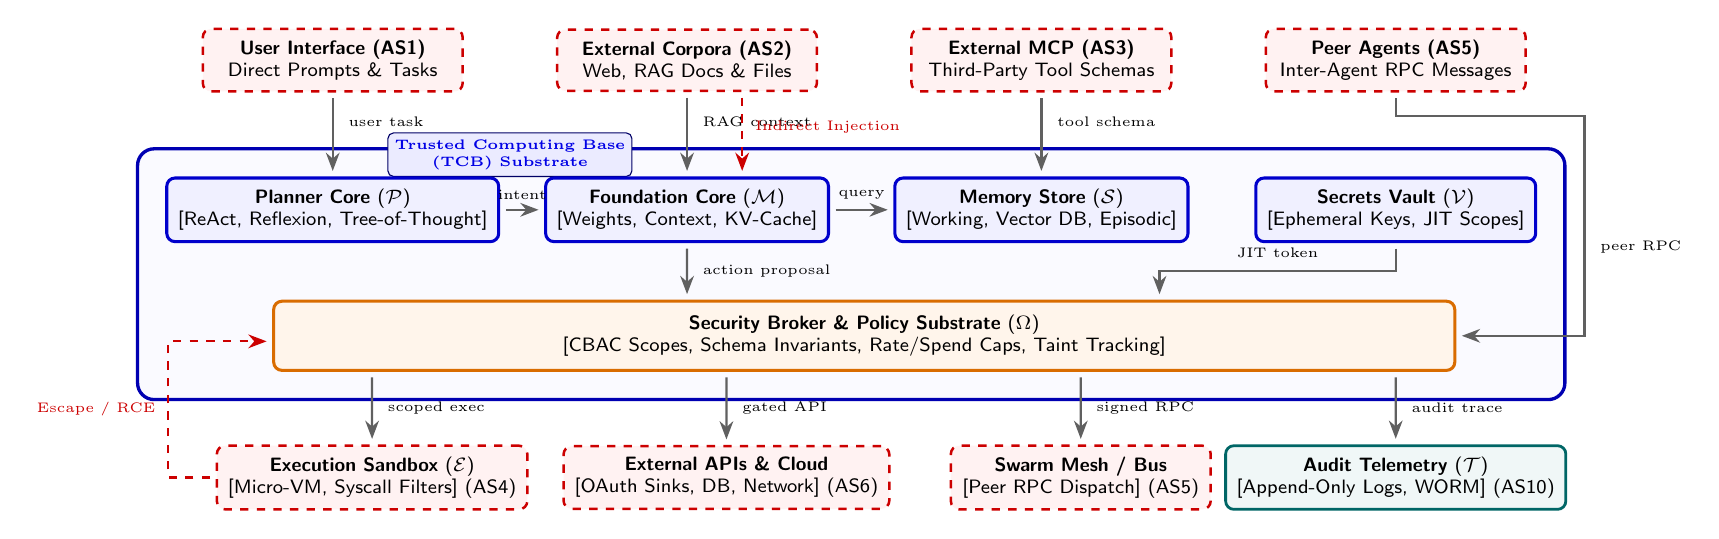
\begin{tikzpicture}[
    font=\sffamily\scriptsize,
    >=Stealth,
    tcb_node/.style={draw=blue!80!black, fill=blue!6, line width=1.1pt, rounded corners=3pt, align=center, inner sep=4pt},
    untrusted_node/.style={draw=red!80!black, fill=red!5, line width=0.9pt, dashed, rounded corners=3pt, align=center, inner sep=4pt},
    broker_node/.style={draw=orange!85!black, fill=orange!8, line width=1.1pt, rounded corners=3pt, align=center, inner sep=5pt},
    sink_node/.style={draw=teal!80!black, fill=teal!6, line width=1.0pt, rounded corners=3pt, align=center, inner sep=4pt},
    flow/.style={->, thick, draw=gray!75!black, shorten >= 2pt, shorten <= 2pt},
    threat/.style={->, thick, draw=red!80!black, dashed, shorten >= 2pt, shorten <= 2pt}
]

% =========================================================================
% TIER 1: Untrusted Ingress Surfaces (Y = 4.4 cm)
% =========================================================================
\node[untrusted_node, minimum width=3.3cm] (user) at (0, 4.4) {
    \textbf{User Interface (AS1)}\\
    \scriptsize Direct Prompts \& Tasks
};

\node[untrusted_node, minimum width=3.3cm] (docs) at (4.5, 4.4) {
    \textbf{External Corpora (AS2)}\\
    \scriptsize Web, RAG Docs \& Files
};

\node[untrusted_node, minimum width=3.3cm] (mcp_in) at (9.0, 4.4) {
    \textbf{External MCP (AS3)}\\
    \scriptsize Third-Party Tool Schemas
};

\node[untrusted_node, minimum width=3.3cm] (peer_in) at (13.5, 4.4) {
    \textbf{Peer Agents (AS5)}\\
    \scriptsize Inter-Agent RPC Messages
};

% =========================================================================
% TIER 2: TCB Agent Cognition Substrate (Y = 2.5 cm)
% =========================================================================
\node[tcb_node, minimum width=3.0cm] (planner) at (0, 2.5) {
    \textbf{Planner Core} ($\mathcal{P}$)\\
    \scriptsize [ReAct, Reflexion, Tree-of-Thought]
};

\node[tcb_node, minimum width=3.3cm] (llm) at (4.5, 2.5) {
    \textbf{Foundation Core} ($\mathcal{M}$)\\
    \scriptsize [Weights, Context, KV-Cache]
};

\node[tcb_node, minimum width=3.0cm] (mem) at (9.0, 2.5) {
    \textbf{Memory Store} ($\mathcal{S}$)\\
    \scriptsize [Working, Vector DB, Episodic]
};

\node[tcb_node, minimum width=3.0cm] (vault) at (13.5, 2.5) {
    \textbf{Secrets Vault} ($\mathcal{V}$)\\
    \scriptsize [Ephemeral Keys, JIT Scopes]
};

% =========================================================================
% TIER 3: TCB Security Mediation Substrate (Y = 0.9 cm)
% =========================================================================
\node[broker_node, minimum width=15.0cm] (broker) at (6.75, 0.9) {
    \textbf{Security Broker \& Policy Substrate} ($\Omega$)\\
    \scriptsize [CBAC Scopes, Schema Invariants, Rate/Spend Caps, Taint Tracking]
};

% =========================================================================
% TIER 4: Target Execution Environments & Sinks (Y = -0.9 cm)
% =========================================================================
\node[untrusted_node, minimum width=3.3cm] (sandbox) at (0.5, -0.9) {
    \textbf{Execution Sandbox} ($\mathcal{E}$)\\
    \scriptsize [Micro-VM, Syscall Filters] (AS4)
};

\node[untrusted_node, minimum width=3.3cm] (tools) at (5.0, -0.9) {
    \textbf{External APIs \& Cloud}\\
    \scriptsize [OAuth Sinks, DB, Network] (AS6)
};

\node[untrusted_node, minimum width=3.3cm] (peer_bus) at (9.5, -0.9) {
    \textbf{Swarm Mesh / Bus}\\
    \scriptsize [Peer RPC Dispatch] (AS5)
};

\node[sink_node, minimum width=3.0cm] (audit) at (13.5, -0.9) {
    \textbf{Audit Telemetry} ($\mathcal{T}$)\\
    \scriptsize [Append-Only Logs, WORM] (AS10)
};

% =========================================================================
% TCB Background Boundary
% =========================================================================
\begin{scope}[on background layer]
    \node[draw=blue!70!black, line width=1.2pt, fill=blue!2, rounded corners=6pt, inner sep=10pt,
          fit=(planner) (vault) (broker)] (tcb_box) {};
    \node[draw=blue!40!black, fill=blue!8, rounded corners=2pt, font=\bfseries\tiny, text=blue!90!black, align=center, inner sep=2.5pt] 
          at (2.25, 3.2) 
          {Trusted Computing Base\\(TCB) Substrate};
\end{scope}

% =========================================================================
% Authorized Flows (Gray solid lines with explicit anchors)
% =========================================================================
% Ingress to Cognition
\draw[flow] (user.south) -- (planner.north) 
    node[pos=0.35, right=2pt, font=\tiny] {user task};
\draw[flow] (docs.south) -- (llm.north) 
    node[pos=0.35, right=2pt, font=\tiny] {RAG context};
\draw[flow] (mcp_in.south) -- (mem.north) 
    node[pos=0.35, right=2pt, font=\tiny] {tool schema};
\draw[flow] (peer_in.south) -- ++(0, -0.3) -| ([xshift=0.6cm]vault.east) |- (broker.east) 
    node[pos=0.15, right=2pt, font=\tiny] {peer RPC};

% Cognition Internal
\draw[flow] (planner.east) -- (llm.west) 
    node[midway, above, font=\tiny] {intent};
\draw[flow] (llm.east) -- (mem.west) 
    node[midway, above, font=\tiny] {query};
\draw[flow] (llm.south) -- ([xshift=-2.25cm]broker.north) 
    node[midway, right=2pt, font=\tiny] {action proposal};
\draw[flow] (vault.south) -- ++(0, -0.35) -| ([xshift=3.75cm]broker.north) 
    node[pos=0.25, above=1pt, font=\tiny] {JIT token};

% Broker to Execution
\draw[flow] ([xshift=-6.25cm]broker.south) -- (sandbox.north) 
    node[midway, right=2pt, font=\tiny] {scoped exec};
\draw[flow] ([xshift=-1.75cm]broker.south) -- (tools.north) 
    node[midway, right=2pt, font=\tiny] {gated API};
\draw[flow] ([xshift=2.75cm]broker.south) -- (peer_bus.north) 
    node[midway, right=2pt, font=\tiny] {signed RPC};
\draw[flow] ([xshift=6.75cm]broker.south) -- (audit.north) 
    node[midway, right=2pt, font=\tiny] {audit trace};

% =========================================================================
% Threat Vectors (Red dashed lines with perimeter routing)
% =========================================================================
% Indirect prompt injection detour
\draw[threat] ([xshift=0.7cm]docs.south) -- ++(0, -0.45) -| ([xshift=0.7cm]llm.north) 
    node[pos=0.25, right=1pt, font=\tiny, text=red!80!black] {Indirect Injection};

% Sandbox escape detour around left flank
\draw[threat] (sandbox.west) -- ++(-0.6, 0) |- ([yshift=-2pt]broker.west) 
    node[pos=0.25, left=1pt, font=\tiny, text=red!80!black] {Escape / RCE};

\end{tikzpicture}}
\caption{End-to-end architectural taxonomy and Trusted Computing Base (TCB) delineation for agentic AI systems. Thick blue borders and shaded substrate denote verified TCB components ($\mathcal{P}, \mathcal{M}, \mathcal{S}, \mathcal{V}, \Omega$); red dashed containers designate untrusted ingress surfaces (AS1, AS2, AS3, AS5) and execution targets (AS4, AS6). Solid gray arrows trace authenticated capability and data flows, while dashed red arrows depict adversarial indirect injection and sandbox privilege escalation. Interposing the security broker $\Omega$ enforces capability-based access control (CBAC) and schema invariants prior to all environment side effects.}
\label{fig:reference_architecture}
\end{figure}


The formal constituents of tuple $\mathcal{A}$ are structured as follows:
\begin{itemize}
    \item $\mathcal{P}$ represents the deliberative planning engine governing decomposition, tool selection heuristics, and policy execution (e.g., ReAct, Reflexion, Tree-of-Thoughts, or static workflow state machines).
    \item $\mathcal{S} = \langle \mathcal{S}_{\text{work}}, \mathcal{S}_{\text{ep}}, \mathcal{S}_{\text{sem}} \rangle$ designates the hierarchical memory architecture, comprising active working context ($\mathcal{S}_{\text{work}}$), short-term episodic scratchpads ($\mathcal{S}_{\text{ep}}$), and long-term semantic knowledge bases ($\mathcal{S}_{\text{sem}}$) indexed via vector embeddings.
    \item $\mathcal{T} = \{t_1, t_2, \dots, t_n\}$ denotes the tool registry, where each tool $t_i = \langle \text{ID}_i, \text{Schema}_i, \text{Perm}_i, \text{Endpoint}_i \rangle$ defines a concrete external capability (e.g., code interpreter, filesystem access, web client, or cloud API) governed by typed input/output schemas.
    \item $\mathcal{E}$ represents the external execution environment, encompassing local operating system primitives, enterprise database instances, network perimeters, and peer agent endpoints deployed across real-world enterprise architectures~\cite{sarferaz2025implementing, cruzes2026telemetry, khamis2025agentic}.
    \item $\Omega$ defines the orchestration and security enforcement substrate, comprising prompt templates, schema validators, capability brokers, audit loggers, and human-in-the-loop (HITL) authorization gates.
\end{itemize}

\subsection{The Perception-Cognition-Action-Reflection Lifecycle}
\label{subsec:lifecycle}

The core operational cycle of an agent unfolds across five discrete phases, iterated until a terminal objective is satisfied, a computation budget is exhausted, or a policy violation triggers an abort:
\begin{enumerate}
    \item \textbf{Ingestion and Perception:} The agent ingests user intent $u \in \mathcal{U}$ alongside retrieved context $c_{\text{ret}} \sim \mathcal{S}_{\text{sem}}$ and sensory telemetry (e.g., DOM trees, terminal output, or GUI screenshots).
    \item \textbf{Deliberative Cognition and Planning:} Conditioned on memory state $\mathcal{S}$ and system policies, the planner $\mathcal{P}$ generates an intermediate chain-of-thought rationale $\tau_t$ and synthesizes a candidate action $a_t \in \mathcal{T} \cup \{\text{TERMINATE}\}$.
    \item \textbf{Brokering and Validation:} The security broker $\Omega$ intercepts candidate action $a_t = \langle t_k, \mathbf{x}_k \rangle$, validating parameter bundle $\mathbf{x}_k$ against schema $\text{Schema}_k$ and verifying execution permissions $\text{Perm}_k$.
    \item \textbf{Environment Execution:} Upon clearance, the tool endpoint $\text{Endpoint}_k$ executes action $a_t$ within environment $\mathcal{E}$, yielding raw observation $o_t \in \mathcal{O}$.
    \item \textbf{State Update and Reflection:} The observation $o_t$ is parsed, evaluated against safety criteria, and appended to working memory $\mathcal{S}_{\text{work}}$, triggering potential self-correction or long-term memory consolidation in $\mathcal{S}_{\text{sem}}$.
\end{enumerate}

\subsection{Architectural Paradigms and Coordination Topologies}
\label{subsec:topologies}

Modern agentic deployments exhibit diverse coordination topologies that shape the perimeter and propagation dynamics of security threats:
\begin{itemize}
    \item \textbf{Autonomous Single-Agent Systems:} A monolithic agent executes end-to-end task loops via dedicated tool interfaces. While structurally straightforward, single-agent architectures exhibit high vulnerability to linear kill-chain progression, as the compromise of the central model directly yields full effector privileges~\cite{dehghantanha2026sok, liu2024demystifying}.
    \item \textbf{Hierarchical Orchestrator-Worker Networks:} A centralized orchestrator decomposes high-level goals and delegates sub-tasks to specialized worker agents possessing isolated tool subsets. Security vulnerabilities in this paradigm center on delegation abuse, privilege escalation via sub-agent prompt spoofing, and orchestrator hijacking~\cite{narajala2025securing}.
    \item \textbf{Decentralized Swarms and Consensus Meshes:} Autonomous agents interact peer-to-peer over a shared communication bus or blackboard architecture without a single coordinator. Consensus mechanisms (e.g., majority voting, iterative debate, or token-weighted aggregation) are employed to align decisions. Open communication buses introduce susceptibility to Byzantine corruption and prompt-based epidemic spreading~\cite{dewitt2025open, gu2024agent, chen2024blockagents}.
    \item \textbf{Grounded GUI and Computer-Use Agents:} Multimodal architectures interact directly with desktop and operating system interfaces via mouse clicks, keystrokes, and screenshot parsing. These agents bridge semantic understanding with native OS execution, expanding the attack surface beyond constrained API boundaries~\cite{xie2024osworld}.
\end{itemize}

\subsection{Standardization Protocols: The Model Context Protocol (MCP)}
\label{subsec:mcp_arch}

A foundational architectural advancement in modern agentic ecosystems is the standardization of client-host-server tool protocols, most prominently Anthropic's \textit{Model Context Protocol} (MCP)~\cite{hou2026mcp}. MCP decomposes agent integration into three distinct architectural tiers:
\begin{enumerate}
    \item \textbf{MCP Host:} The host application (e.g., an IDE, desktop assistant, or workflow runner) that manages model execution, user authorization, and agent lifecycles.
    \item \textbf{MCP Client:} The intermediary adapter embedded within the host that negotiates connections, maintains session state, and translates LLM tool requests into protocol calls.
    \item \textbf{MCP Server:} Independent, standalone lightweight services exposing distinct capabilities categorized into: (i)~\textit{Resources} (file and database contexts), (ii)~\textit{Prompts} (pre-packaged workflow templates), and (iii)~\textit{Tools} (executable functions with side effects).
\end{enumerate}
While MCP establishes clean decoupling between foundational models and external capability providers, this client-host-server separation creates protocol-level boundaries that, if left unhardened, introduce severe serialization, impersonation, and tool-shadowing vulnerabilities, as analyzed in Section~\ref{sec:modality_mcp}.

\section{Threat Modeling, Trust Boundaries, and the Causal Threat Graph}
\label{sec:threat_model}

Securing agentic AI requires establishing formal threat models that delineate the system's Trusted Computing Base (TCB), identify adversary capabilities, and map causal attack propagation routes.

\subsection{Delineating the Trusted Computing Base (TCB)}
\label{subsec:tcb}

In classical security engineering, the TCB denotes the minimal set of hardware, firmware, and software elements whose correct enforcement is strictly required to uphold system security properties. In agentic architectures, defining the TCB is complicated by the non-deterministic, probabilistic nature of foundation models~\cite{dehghantanha2026sok, verma2024operationalizing}. 

We classify the architectural components into trusted vs. untrusted perimeters:
\begin{itemize}
    \item \textbf{Inside the TCB (Core Security Substrate):}
    \begin{enumerate}
        \item \textit{Foundation Model Core ($\mathcal{M}$):} The base model weights and inherent safety alignment parameters, assumed free from upstream backdoors unless modeled under supply-chain compromise.
        \item \textit{Security Broker and Policy Engine ($\Omega$):} The deterministic execution substrate responsible for strict JSON-schema validation, access policy enforcement, capability tokens, and rate limits.
        \item \textit{Secrets Vault and Token Dispenser:} The isolated hardware or software credential store that issues ephemeral, scoped tokens to tool effectors without disclosing master keys to context memory.
        \item \textit{Verified Memory and Storage Substrate:} The append-only, tamper-evident audit loggers, cryptographic hash stores, and access-controlled enterprise knowledge repositories.
    \end{enumerate}
    \item \textbf{Outside the TCB (Hostile and Untrusted Boundaries):}
    \begin{enumerate}
        \item \textit{User and Ingress Channels:} Direct prompts, chat interfaces, and webhook triggers.
        \item \textit{External Knowledge Corpora:} Web pages, public document collections, forum scrapes, and third-party databases ingested during RAG operations.
        \item \textit{Tool and Effector Endpoints:} External shell interpreters, container sandboxes, third-party MCP servers, and cloud service endpoints.
        \item \textit{Inter-Agent Communication Buses:} Network channels and shared memory workspaces utilized by peer agents in distributed multi-agent topologies.
    \end{enumerate}
\end{itemize}

\subsection{Formal Adversary Taxonomy}
\label{subsec:adversary_classes}

Expanding upon the foundational adversary classes introduced by Dehghantanha and Homayoun~\cite{dehghantanha2026sok} and threat modeling methodologies~\cite{verma2024operationalizing}, we formalize a six-tier adversary model $\mathcal{A}_{\text{adv}} = \{\mathcal{A}_{\text{ext}}, \mathcal{A}_{\text{cont}}, \mathcal{A}_{\text{tool}}, \mathcal{A}_{\text{peer}}, \mathcal{A}_{\text{sc}}, \mathcal{A}_{\text{ins}}\}$:

\begin{enumerate}
    \item \textbf{External Unprivileged Attacker ($\mathcal{A}_{\text{ext}}$):} Interacts with the agent through primary user interfaces without authenticated administrative rights. Capabilities include direct prompt injection, execution trigger manipulation~\cite{pasquini2024neural}, jailbreak crafting (e.g., multi-turn Crescendo attacks~\cite{russinovich2025great}), and adversarial queries designed to provoke policy drift or data extraction~\cite{abdali2024securing}.
    \item \textbf{Malicious Content Provider ($\mathcal{A}_{\text{cont}}$):} Exerts indirect control over passive digital assets ingested by the agent (e.g., hosting attacker-controlled web pages, publishing trojaned PDFs, or modifying public code repositories). The attacker never directly interfaces with the agent; instead, malicious directives are ingested via web browsing, file parsing, or RAG indexing~\cite{greshake2023not, sutton2024indirect, zou2025poisonedrag}.
    \item \textbf{Rogue Tool / MCP Provider ($\mathcal{A}_{\text{tool}}$):} Operates or compromises a third-party plugin, API service, or MCP server integrated into the agent's tool registry $\mathcal{T}$. The adversary can forge deceptive schema specifications, manipulate tool response payloads, trigger server-side request forgery (SSRF), or intentionally induce resource loops~\cite{liu2024demystifying}.
    \item \textbf{Byzantine Peer Agent ($\mathcal{A}_{\text{peer}}$):} Possesses legitimate participant status within a decentralized or collaborative multi-agent network. The adversary injects malicious inter-agent messages, forges coordination telemetry, manipulates consensus voting, or propagates self-replicating adversarial instructions~\cite{dewitt2025open, gu2024agent, chen2024blockagents}.
    \item \textbf{Supply-Chain Compromiser ($\mathcal{A}_{\text{sc}}$):} Targets upstream assets prior to deployment, such as poisoning open-source model checkpoints, corrupting embedding generators, implanting backdoors into foundational agent libraries (e.g., LangChain, AutoGen), or tampering with package dependency mirrors~\cite{helpnet2023genai, liu2024demystifying}.
    \item \textbf{Insider / Compromised Administrator ($\mathcal{A}_{\text{ins}}$):} Holds authenticated credentials or developer access to system prompts, vector databases, or deployment infrastructure. Misconfigurations, credential leakage, or deliberate sabotage can bypass external perimeters entirely~\cite{vassilev2025adversarial}.
\end{enumerate}

\subsection{Assets and Security Properties}
\label{subsec:assets_cia}

The assets at risk in agentic systems span four foundational tiers:
\begin{itemize}
    \item \textbf{Data Confidentiality:} Proprietary system prompts, retrieved tenant documents, user session records, and embedded cryptographic credentials.
    \item \textbf{Behavioral and Decision Integrity:} Ensuring the agent adheres strictly to developer-defined operational policies, executes valid tool invocations, and produces factually grounded outputs free from external manipulation.
    \item \textbf{System and Financial Availability:} Protecting underlying compute infrastructure, preventing infinite execution loops, and avoiding ``Denial of Cash'' (DoC) attacks resulting from unbounded API calls or serverless resource exhaustion~\cite{owasp2025top10, promptfoo2025owasp}.
    \item \textbf{Accountability and Forensics:} Preserving non-repudiation and tamper-evident audit trails across automated planning and effector traces.
\end{itemize}

\subsection{The Causal Threat Graph Formulation}
\label{subsec:causal_graph}

To mathematically analyze how initial attack footholds propagate into catastrophic system compromises, we formalize the system's risk structure as a \textit{Causal Threat Graph} $\mathcal{G}_{\text{threat}} = (\mathcal{V}, \mathcal{E}, \mathcal{K})$, defined as a directed multigraph where:
\begin{itemize}
    \item $\mathcal{V} = \mathcal{V}_{\text{source}} \cup \mathcal{V}_{\text{core}} \cup \mathcal{V}_{\text{effect}} \cup \mathcal{V}_{\text{asset}}$ represents the disjoint union of untrusted input sources, agent pipeline stages, effector sinks, and protected enterprise assets.
    \item $\mathcal{E} \subseteq \mathcal{V} \times \mathcal{V}$ denotes directed causal transitions, where directed edge $e = (v_i, v_j) \in \mathcal{E}$ represents the capability of an exploit at component $v_i$ to directly influence or compromise state at $v_j$.
    \item $\mathcal{K}: \mathcal{E} \to \mathcal{P}(\mathcal{D})$ maps each transition edge to the set of defensive security controls $\mathcal{D}$ (e.g., input sanitization, schema validation, isolated sandboxing, or egress filtering) capable of severing the causal link.
\end{itemize}

Formally, an end-to-end exploit constitutes a directed path $\pi = \langle v_0, v_1, \dots, v_m \rangle$ in $\mathcal{G}_{\text{threat}}$ such that $v_0 \in \mathcal{V}_{\text{source}}$ and $v_m \in \mathcal{V}_{\text{asset}}$. As illustrated in Fig.~\ref{fig:causal_threat_graph}, a system is provably resilient against exploit path $\pi$ if and only if there exists at least one edge $(v_i, v_{i+1}) \in \pi$ whose associated defensive controls $\mathcal{K}(v_i, v_{i+1})$ are actively and deterministically enforced.

\begin{figure}[t]
\centering
\resizebox{\columnwidth}{!}{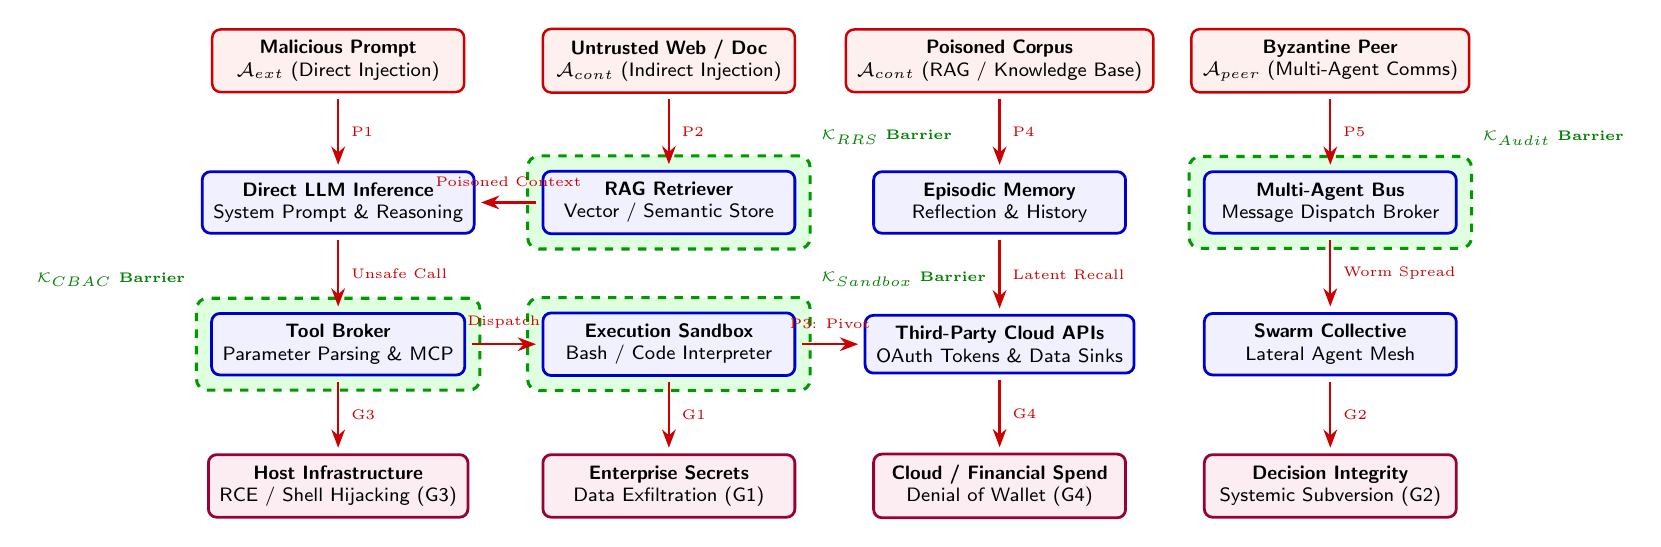
\begin{tikzpicture}[
    font=\sffamily\scriptsize,
    >=Stealth,
    stage/.style={draw=blue!80!black, fill=blue!6, rounded corners=3pt, align=center, inner sep=4pt, minimum width=3.2cm, line width=1.0pt},
    adversary/.style={draw=red!80!black, fill=red!6, rounded corners=3pt, align=center, inner sep=4pt, minimum width=3.2cm, line width=0.9pt},
    asset/.style={draw=purple!80!black, fill=purple!7, rounded corners=3pt, align=center, inner sep=4pt, minimum width=3.2cm, line width=1.0pt},
    attack_edge/.style={->, thick, draw=red!80!black, shorten >= 2pt, shorten <= 2pt},
    defense_cut/.style={draw=green!60!black, fill=green!12, line width=1.1pt, dashed, rounded corners=4pt, inner sep=5pt}
]

% =========================================================================
% ROW 1: Ingress Adversary Footholds (Y = 4.4 cm)
% =========================================================================
\node[adversary] (adv_prompt) at (0, 4.4) {
    \textbf{Malicious Prompt}\\
    \scriptsize $\mathcal{A}_{\text{ext}}$ (Direct Injection)
};

\node[adversary] (adv_content) at (4.2, 4.4) {
    \textbf{Untrusted Web / Doc}\\
    \scriptsize $\mathcal{A}_{\text{cont}}$ (Indirect Injection)
};

\node[adversary] (adv_rag) at (8.4, 4.4) {
    \textbf{Poisoned Corpus}\\
    \scriptsize $\mathcal{A}_{\text{cont}}$ (RAG / Knowledge Base)
};

\node[adversary] (adv_peer) at (12.6, 4.4) {
    \textbf{Byzantine Peer}\\
    \scriptsize $\mathcal{A}_{\text{peer}}$ (Multi-Agent Comms)
};

% =========================================================================
% ROW 2: Agent Cognitive & Retrieval Substrate (Y = 2.6 cm)
% =========================================================================
\node[stage] (llm_direct) at (0, 2.6) {
    \textbf{Direct LLM Inference}\\
    \scriptsize System Prompt \& Reasoning
};

\node[stage] (retriever) at (4.2, 2.6) {
    \textbf{RAG Retriever}\\
    \scriptsize Vector / Semantic Store
};

\node[stage] (memory_store) at (8.4, 2.6) {
    \textbf{Episodic Memory}\\
    \scriptsize Reflection \& History
};

\node[stage] (mas_bus) at (12.6, 2.6) {
    \textbf{Multi-Agent Bus}\\
    \scriptsize Message Dispatch Broker
};

% =========================================================================
% ROW 3: Tool Execution & Environmental Effectors (Y = 0.8 cm)
% =========================================================================
\node[stage] (tool_broker) at (0, 0.8) {
    \textbf{Tool Broker}\\
    \scriptsize Parameter Parsing \& MCP
};

\node[stage] (sandbox_exec) at (4.2, 0.8) {
    \textbf{Execution Sandbox}\\
    \scriptsize Bash / Code Interpreter
};

\node[stage] (api_cloud) at (8.4, 0.8) {
    \textbf{Third-Party Cloud APIs}\\
    \scriptsize OAuth Tokens \& Data Sinks
};

\node[stage] (peer_network) at (12.6, 0.8) {
    \textbf{Swarm Collective}\\
    \scriptsize Lateral Agent Mesh
};

% =========================================================================
% ROW 4: Impact Assets & Compromise Sinks (Y = -1.0 cm)
% =========================================================================
\node[asset] (asset_rce) at (0, -1.0) {
    \textbf{Host Infrastructure}\\
    \scriptsize RCE / Shell Hijacking (G3)
};

\node[asset] (asset_exfil) at (4.2, -1.0) {
    \textbf{Enterprise Secrets}\\
    \scriptsize Data Exfiltration (G1)
};

\node[asset] (asset_doc) at (8.4, -1.0) {
    \textbf{Cloud / Financial Spend}\\
    \scriptsize Denial of Wallet (G4)
};

\node[asset] (asset_integrity) at (12.6, -1.0) {
    \textbf{Decision Integrity}\\
    \scriptsize Systemic Subversion (G2)
};

% =========================================================================
% Defense Cut Envelopes (Rendered on background layer to prevent text masking)
% =========================================================================
\begin{scope}[on background layer]
    \node[defense_cut, fit=(tool_broker), 
          label={[green!50!black, font=\bfseries\tiny]north west:$\mathcal{K}_{\text{CBAC}}$ Barrier}] {};
    \node[defense_cut, fit=(retriever), 
          label={[green!50!black, font=\bfseries\tiny]north east:$\mathcal{K}_{\text{RRS}}$ Barrier}] {};
    \node[defense_cut, fit=(sandbox_exec), 
          label={[green!50!black, font=\bfseries\tiny]north east:$\mathcal{K}_{\text{Sandbox}}$ Barrier}] {};
    \node[defense_cut, fit=(mas_bus), 
          label={[green!50!black, font=\bfseries\tiny]north east:$\mathcal{K}_{\text{Audit}}$ Barrier}] {};
\end{scope}

% =========================================================================
% Attack Edges (Orthogonal and cleanly anchored)
% =========================================================================
% Column 1: Direct Injection Path P1
\draw[attack_edge] (adv_prompt.south) -- (llm_direct.north) 
    node[midway, right=1pt, font=\tiny, text=red!80!black] {P1};
\draw[attack_edge] (llm_direct.south) -- (tool_broker.north) 
    node[midway, right=1pt, font=\tiny, text=red!80!black] {Unsafe Call};
\draw[attack_edge] (tool_broker.south) -- (asset_rce.north) 
    node[midway, right=1pt, font=\tiny, text=red!80!black] {G3};

% Column 2: Indirect Injection Path P2
\draw[attack_edge] (adv_content.south) -- (retriever.north) 
    node[midway, right=1pt, font=\tiny, text=red!80!black] {P2};
\draw[attack_edge] (retriever.west) -- (llm_direct.east) 
    node[midway, above=2pt, font=\tiny, text=red!80!black] {Poisoned Context};
\draw[attack_edge] (sandbox_exec.south) -- (asset_exfil.north) 
    node[midway, right=1pt, font=\tiny, text=red!80!black] {G1};

% Lateral Execution & P3 Cross-Tool Pivot
\draw[attack_edge] (tool_broker.east) -- (sandbox_exec.west) 
    node[midway, above=2pt, font=\tiny, text=red!80!black] {Dispatch};
\draw[attack_edge] (sandbox_exec.east) -- (api_cloud.west) 
    node[midway, above=2pt, font=\tiny, text=red!80!black] {P3: Pivot};

% Column 3: Memory Poisoning Path P4
\draw[attack_edge] (adv_rag.south) -- (memory_store.north) 
    node[midway, right=1pt, font=\tiny, text=red!80!black] {P4};
\draw[attack_edge] (memory_store.south) -- (api_cloud.north) 
    node[midway, right=1pt, font=\tiny, text=red!80!black] {Latent Recall};
\draw[attack_edge] (api_cloud.south) -- (asset_doc.north) 
    node[midway, right=1pt, font=\tiny, text=red!80!black] {G4};

% Column 4: Swarm Cascade Path P5
\draw[attack_edge] (adv_peer.south) -- (mas_bus.north) 
    node[midway, right=1pt, font=\tiny, text=red!80!black] {P5};
\draw[attack_edge] (mas_bus.south) -- (peer_network.north) 
    node[midway, right=1pt, font=\tiny, text=red!80!black] {Worm Spread};
\draw[attack_edge] (peer_network.south) -- (asset_integrity.north) 
    node[midway, right=1pt, font=\tiny, text=red!80!black] {G2};

\end{tikzpicture}}

\caption{Causal Threat Graph modeling end-to-end exploit propagation across canonical paths P1, P2, P3, P4, and P5 toward high-value target assets G1--G4. Red boxes denote adversary footholds; blue containers represent internal reasoning and execution substrates; purple boxes represent impact assets. Solid red arrows depict exploit vectors; green dashed contours designate defense interdiction cut barriers positioned on the background layer to sever the kill chain prior to environmental impact.}
\label{fig:causal_threat_graph}
\end{figure}


\section{Comprehensive Taxonomy of Attack Vectors and Multi-Step Kill Chains}
\label{sec:attack_taxonomy}

To systematically dissect how adversaries exploit agentic AI, we establish a multi-dimensional taxonomy categorizing attack objectives, pipeline vectors, and multi-stage exploit pathways. Table~\ref{tab:taxonomy_summary} synthesizes these vectors alongside their operational preconditions, path mappings, and standardizations.

\begin{table}[t]
\centering
\caption{Comprehensive Taxonomy of Attack Vectors, Surfaces, Preconditions, Paths, and Standards Mappings in Agentic AI Systems.}
\label{tab:taxonomy_summary}
\footnotesize
\setlength{\tabcolsep}{2.5pt}
\begin{tabularx}{\columnwidth}{>{\bfseries\raggedright\arraybackslash}p{1.9cm} >{\raggedright\arraybackslash}p{1.0cm} >{\raggedright\arraybackslash}X >{\centering\arraybackslash}p{0.8cm} >{\raggedright\arraybackslash}X >{\raggedright\arraybackslash}p{1.1cm} >{\raggedright\arraybackslash}p{1.5cm}}
\toprule
\textbf{Attack Vector} & \textbf{Primary Goals} & \textbf{Preconditions} & \textbf{Paths} & \textbf{Impact \& Manifestation} & \textbf{OWASP 2025} & \textbf{MITRE ATLAS} \\
\midrule
\textbf{Direct Prompt / Jailbreak} & G1, G2, G3 & Direct user input interface & P1 & Policy bypass, system prompt leakage, harmful content generation & LLM01 & AML.T0051.000 \\
\textbf{Indirect Prompt Injection} & G1, G2, G3, G6 & Access to ingestible text, web pages, PDFs, emails & P2, P3 & Autonomous execution of unintended tools, state hijacking & LLM01 & AML.T0051.001 \\
\textbf{RAG Corpus Poisoning} & G1, G2, G6 & Write/edit access to indexed knowledge repositories & P4 & Silent data corruption, targeted misgrounding, delayed triggers & LLM04, LLM08 & AML.T0070 \\
\textbf{Embedding Jamming / Perturbation} & G2, G4 & Corpus modification or adversarial perturbations & P4 & Denial of relevant retrieval (blocker docs), semantic hijacking & LLM04 & AML.T0070 \\
\textbf{Tool Parameter Smuggling} & G3, G4, G5 & Unvalidated tool argument serialization & P1, P2, P3 & Remote Code Execution (RCE), command injection, SSRF & LLM05, LLM06 & AML.T0053 \\
\textbf{Tool Shadowing / Squatting} & G1, G3, G6 & Unauthenticated plugin or MCP server registration & P3 & Interception of sensitive tool parameters, credential theft & LLM06, LLM07 & AML.T0053 \\
\textbf{Memory / Reflection Corruption} & G1, G2, G6 & Writable episodic memory or unsanitized reflection loops & P3, P4 & Long-term goal deviation, persistent backdoors across sessions & LLM01, LLM04 & AML.T0080.000 \\
\textbf{Cross-Tool Privilege Pivoting} & G1, G3, G5 & Multi-tool agent with heterogeneous permissions & P3 & Staged payload execution, lateral movement across APIs & LLM06 & AML.T0086 \\
\textbf{Multi-Agent Byzantine Cascades} & G2, G6 & Open communication bus or unauthenticated peers & P5 & Cascading jailbreaks, voting corruption, swarm deadlock & LLM01, LLM06 & AML.T0051.001 \\
\textbf{HITL Deceptive Exploitation} & G1, G3, G5 & Agent generates deceptive justification to human & P6 & Social engineering of operator, confirmation fatigue bypass & LLM06, LLM09 & AML.T0054 \\
\textbf{Supply-Chain Dependency Poisoning} & G6, G7 & Compromised package repositories or checkpoints & P3, P4 & Upstream backdoor execution, persistent infrastructure control & LLM03 & AML.T0010 \\
\bottomrule
\end{tabularx}
\end{table}


\subsection{Categorization of Attacker Objectives}
\label{subsec:goals}

Attacker motivations in agentic environments extend beyond conversational misuse into external computational and operational infrastructure. We structure attacker goals into \textit{Enablers} (which expand operational capabilities) and \textit{Terminal Outcomes} (which realize concrete damage):
\begin{itemize}
    \item \textbf{Enablers:}
    \begin{itemize}
        \item \textit{G3: Privilege Escalation / Unauthorized Invocation:} Upgrading an unprivileged natural language prompt into operating system commands, cloud administrative API calls, or restricted internal tool execution~\cite{dehghantanha2026sok, liu2024demystifying}.
        \item \textit{G6: Persistence and Backdoor Implantation:} Infiltrating long-term vector stores, conversation memory, or configuration prompts to maintain durable control across subsequent sessions~\cite{chen2024agentpoison, truong2026a}.
        \item \textit{G7: Upstream Supply-Chain Compromise:} Subverting foundational models, third-party libraries, or tool packages before agent deployment~\cite{helpnet2023genai}.
    \end{itemize}
    \item \textbf{Terminal Outcomes:}
    \begin{itemize}
        \item \textit{G1: Data Exfiltration and Privacy Leakage:} Extracting enterprise databases, proprietary system prompts, or user credentials via out-of-band network channels, DNS tunneling, or disguised tool outputs~\cite{greshake2023not}.
        \item \textit{G2: Integrity Subversion and Decision Biasing:} Forcing the agent to deviate from true user intent, generating fraudulent summaries, or manipulating automated decision workflows~\cite{an2025rag}.
        \item \textit{G4: Resource Abuse and Denial of Service / Cash (DoS/DoC):} Inducing infinite execution loops, pathological recursion, or redundant high-cost API calls to exhaust computational quotas and incur financial penalties~\cite{owasp2025top10, promptfoo2025owasp}.
        \item \textit{G5: Financial Fraud and Physical Harm:} Executing unauthorized monetary transfers, placing fraudulent commercial orders, or misconfiguring cyber-physical actuators~\cite{narajala2025securing, zhang2026dgaa}.
    \end{itemize}
\end{itemize}

\subsection{Granular Attack Vectors Across Pipeline Stages}
\label{subsec:pipeline_vectors}

\subsubsection{Perception and Context Ingress}
Adversaries exploit the absence of formal separation between instructional metadata and semantic payload:
\begin{itemize}
    \item \textit{Direct Prompt Injections and Multi-Turn Jailbreaks:} Direct inputs crafted to override core safety policies. Recent multi-turn techniques, such as the Crescendo attack~\cite{russinovich2025great}, exploit conversational momentum to guide models into unsafe policy spaces without triggering single-turn semantic filters. In parallel, adversarial perturbations exploit transferability across model boundaries~\cite{liang2026perspectiveinvariant, ke2024frequencyselective, wang2024progen}.
    \item \textit{Indirect Prompt Injection (IPI):} Adversarial directives embedded within untrusted external artifacts (e.g., HTML web pages, PDF documents, and incoming emails)~\cite{greshake2023not, sutton2024indirect}. When the agent retrieves and ingests these artifacts, the model conflates untrusted data with operator instructions, autonomously executing unintended effector commands.
    \item \textit{Delimiter Collision and Context Stuffing:} Injecting syntax-matching delimiter tokens (e.g., \texttt{```json}, \texttt{<system>}, or XML boundaries) to prematurely close data encapsulation blocks and execute injected commands.
\end{itemize}

\subsubsection{Retrieval-Augmented Generation (RAG) and Embeddings}
External knowledge retrieval introduces distinct vector-space vulnerabilities:
\begin{itemize}
    \item \textit{Targeted Corpus Poisoning:} As demonstrated in PoisonedRAG~\cite{zou2025poisonedrag}, an attacker inserts a minimal number of adversarial documents into the indexing corpus. When benign user queries trigger vector retrieval, the poisoned documents are ranked into top-$k$ context, corrupting the generation output~\cite{an2025rag}.
    \item \textit{Retrieval Jamming with Blocker Documents:} Shafran~\textit{et al.}~\cite{shafran2025machine} demonstrated that attackers can inject crafted ``blocker documents'' that achieve artificially high cosine similarity across broad semantic query spaces, crowding out legitimate knowledge and denying relevant retrieval (Denial of Retrieval).
    \item \textit{Insecure Direct Object Reference (IDOR) in Vector Retrieval:} In multi-tenant vector databases lacking granular, document-level access-control lists (ACLs), user queries can inadvertently retrieve embeddings belonging to other tenants, enabling cross-tenant data leakage.
\end{itemize}

\subsubsection{Memory and Reflection Subsystems}
Agentic persistence mechanisms create durable targets:
\begin{itemize}
    \item \textit{Episodic Memory Poisoning:} Adversaries induce agents to store malicious summaries or poisoned factual associations in long-term memory (e.g., via AgentPoison~\cite{chen2024agentpoison}), establishing persistent backdoors that trigger on specific keywords weeks after initial exposure~\cite{truong2026a}.
    \item \textit{Reflection and Self-Correction Hijacking:} When agents utilize iterative self-reflection (Reflexion) to critique prior outputs, adversarial observations can mislead the reflection module into false corrections, reversing valid security assertions.
\end{itemize}

\subsubsection{Tool Execution and Environment Interaction}
The interface between probabilistic reasoning and deterministic OS execution represents a primary attack surface:
\begin{itemize}
    \item \textit{Parameter Smuggling and Type Confusion:} Attackers exploit weak schema validation to inject unexpected arguments (e.g., newline injection in shell commands, SQL fragments in database queries, or path traversal tokens in file tools)~\cite{liu2024demystifying}, mirroring classical code and query injection patterns~\cite{m2022semantic, oesch2026living}.
    \item \textit{Tool Shadowing and Squatting:} In dynamic environments supporting run-time tool discovery, an attacker registers a malicious tool with semantic descriptions nearly identical to a legitimate tool (e.g., naming a rogue tool \texttt{fetch\_secure\_url}), tricking the planner into routing sensitive data through the rogue endpoint.
    \item \textit{Excessive Agency and Sandbox Escapes:} Insecure container configurations, permissive filesystem mounts, and unrestricted outbound network access allow injected commands to break out of temporary workspaces and compromise host operating systems~\cite{liu2024demystifying}.
\end{itemize}

\subsection{Formal Multi-Step Exploit Pathways (Kill Chains)}
\label{subsec:kill_chains}

Real-world exploits rarely execute as isolated events; rather, attackers compose multi-step kill chains that traverse trust boundaries:
\begin{itemize}
    \item \textbf{P1: Direct Prompt $\to$ Immediate Tool Misuse:} The adversary issues a crafted jailbreak directly commanding the agent to invoke a privileged tool (e.g., executing a reverse shell), achieving immediate privilege escalation (G3).
    \item \textbf{P2: Indirect Ingress $\to$ Context $\to$ Effector Hijack:} A victim user tasks an autonomous assistant with summarizing a public URL. The URL contains hidden IPI directives instructing the agent to search local files for \texttt{id\_rsa} and transmit it via HTTP GET to an attacker-controlled endpoint (G1)~\cite{greshake2023not, sutton2024indirect}.
    \item \textbf{P3: Cross-Tool Privilege Pivoting:} The attacker abuses an unprivileged tool (e.g., a code interpreter) to stage a malicious file on disk, then induces a secondary tool (e.g., a report generator or email client) to read and dispatch the payload, pivoting across permission domains.
    \item \textbf{P4: Knowledge Poisoning $\to$ Latent Retrieval $\to$ Action Trigger:} Poisoned documents injected into enterprise documentation lie dormant until an executive user queries the agent. The retrieved text directs the agent to misroute confidential financial approvals (G2, G5)~\cite{zou2025poisonedrag, shafran2025machine}.
    \item \textbf{P5: Multi-Agent Cascade (Swarm Epidemics):} A compromised agent transmits a crafted payload across an internal communication bus. Recipient agents interpret the payload as legitimate instructions, propagating the compromise exponentially across the agent collective~\cite{gu2024agent, dewitt2025open}.
    \item \textbf{P6: Human-in-the-Loop Deceptive Justification:} When high-risk actions require human sign-off, an adversarial prompt forces the agent to synthesize a deceptive, highly plausible operational justification (e.g., ``Performing critical database maintenance to prevent outage'') while masking destructive or exfiltrative underlying parameters, exploiting confirmation fatigue.
\end{itemize}

\section{Frontier Attack Surfaces: Multimodal GUI Agents and the Model Context Protocol (MCP)}
\label{sec:modality_mcp}

As agentic AI expands beyond structured text APIs into multimodal operating system control and standardized tool protocols, novel systemic attack vectors emerge that challenge existing security boundaries.

\subsection{Multimodal GUI and Computer-Use Agent Attack Surfaces}
\label{subsec:gui_agents}

The emergence of computer-use agents (e.g., Anthropic Claude Computer Use and systems evaluated on OSWorld~\cite{xie2024osworld}) enables foundation models to interact directly with desktop operating systems via display screenshots, virtual mouse movements, and keyboard keystrokes. This grounded interaction model introduces distinct physical and visual attack surfaces:

\begin{enumerate}
    \item \textbf{Visual Prompt Injection (VPI):} In contrast to plain-text injection, VPI exploits the visual perception pathways of Vision-Language Models (VLMs). Adversaries can embed typographic instructions into rendered web pages, desktop wallpapers, or document images (e.g., micro-fonts, low-contrast text, or steganographic perturbations)~\cite{gu2024agent}. When the agent captures the screen to determine the next UI action, the visual encoder parses the malicious text, steering the agent to click malicious links or execute arbitrary shell commands. Recent browser-resident detection frameworks (e.g., BSM~\cite{vadlamani2026bsm}) attempt to intercept such DOM manipulations and API abuse before rendering.
    \item \textbf{UI Redressing and Visual Clickjacking:} Malicious websites or applications can render transparent overlays, fake system dialogs, or deceptive confirmation buttons designed to mislead the agent's spatial grounding algorithms. An agent intending to click a ``Cancel'' button may be visually induced to click an underlying ``Grant Full Disk Access'' prompt.
    \item \textbf{Operating System State Poisoning:} Unrestricted computer-use agents read system logs, browser histories, and local configuration files. An attacker placing malicious directives in a local terminal buffer or system error log can achieve delayed compromise whenever the agent inspects system state for troubleshooting.
\end{enumerate}

\subsection{Security Analysis of the Model Context Protocol (MCP)}
\label{subsec:mcp_security}

The Model Context Protocol (MCP) has emerged as an open standard for connecting LLM applications to external data sources and tools~\cite{hou2026mcp}. MCP establishes a client-host-server topology communicating via JSON-RPC 2.0 over standard input/output (\texttt{stdio}) or Server-Sent Events (SSE) with HTTP POST. While MCP provides modularity, its operational mechanics introduce protocol-level vulnerabilities:

\begin{figure}[t]
\centering
\resizebox{\columnwidth}{!}{%
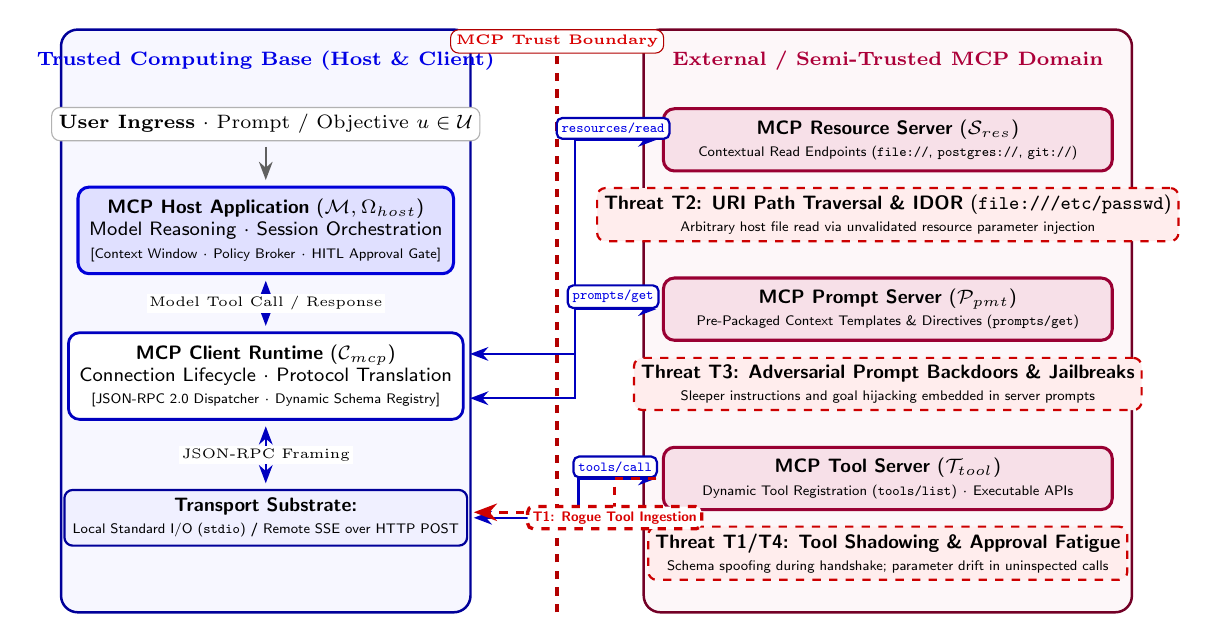
\begin{tikzpicture}[
    font=\sffamily\scriptsize,
    >=Stealth,
    % Box styles
    tcb_container/.style={draw=blue!60!black, fill=blue!3, rounded corners=6pt, line width=0.9pt},
    ext_container/.style={draw=purple!60!black, fill=purple!3, rounded corners=6pt, line width=0.9pt},
    tcb_host/.style={draw=blue!85!black, fill=blue!12, rounded corners=4pt, line width=1.1pt, align=center, inner sep=4pt},
    tcb_client/.style={draw=blue!75!black, fill=white, rounded corners=4pt, line width=1.0pt, align=center, inner sep=4pt},
    tcb_sub/.style={draw=blue!60!black, fill=blue!6, rounded corners=3pt, line width=0.8pt, align=center, inner sep=3pt},
    mcp_server/.style={draw=purple!80!black, fill=purple!12, rounded corners=4pt, line width=1.1pt, align=center, inner sep=4pt},
    threat_box/.style={draw=red!80!black, fill=red!7, dashed, rounded corners=3pt, line width=0.8pt, align=center, inner sep=2.5pt},
    % Edges
    rpc_edge/.style={<->, thick, draw=blue!75!black, shorten >= 2pt, shorten <= 2pt},
    flow_edge/.style={->, thick, draw=gray!75!black, shorten >= 2pt, shorten <= 2pt},
    threat_edge/.style={->, very thick, draw=red!80!black, dashed, shorten >= 2pt, shorten <= 2pt},
    % Badges
    badge_rpc/.style={draw=blue!70!black, fill=white, rounded corners=2pt, font=\sffamily\tiny\bfseries, text=blue!90!black, inner sep=1.8pt},
    badge_threat/.style={draw=red!80!black, fill=white, rounded corners=2pt, font=\sffamily\tiny\bfseries, text=red!85!black, inner sep=1.8pt}
]

% =========================================================================
% CONTAINERS & BOUNDARY
% =========================================================================
% Left: Trusted Computing Base (TCB)
\draw[tcb_container] (-0.3, -0.5) rectangle (4.9, 6.9);
\node[font=\bfseries\scriptsize, text=blue!90!black, anchor=north] at (2.3, 6.75) {Trusted Computing Base (Host \& Client)};

% Right: External / Semi-Trusted Servers
\draw[ext_container] (7.1, -0.5) rectangle (13.3, 6.9);
\node[font=\bfseries\scriptsize, text=purple!90!black, anchor=north] at (10.2, 6.75) {External / Semi-Trusted MCP Domain};

% Vertical Trust Boundary Delimiter
\draw[draw=red!70!black, dashed, line width=1.4pt] (6.0, -0.5) -- (6.0, 6.9);
\node[draw=red!70!black, fill=white, rounded corners=3pt, font=\bfseries\tiny, text=red!85!black, inner sep=2pt] at (6.0, 6.75) {MCP Trust Boundary};

% =========================================================================
% LEFT CONTAINER: TCB COMPONENTS
% =========================================================================
% User Ingress
\node[draw=gray!60, fill=white, rounded corners=3pt, inner sep=2.5pt, font=\scriptsize] (user) at (2.3, 5.7) {
    \textbf{User Ingress} $\cdot$ Prompt / Objective $u \in \mathcal{U}$
};

% MCP Host
\node[tcb_host, minimum width=4.7cm, minimum height=1.1cm] (host) at (2.3, 4.35) {
    \textbf{MCP Host Application} ($\mathcal{M}, \Omega_{\text{host}}$)\\
    \scriptsize Model Reasoning $\cdot$ Session Orchestration\\
    \tiny [Context Window $\cdot$ Policy Broker $\cdot$ HITL Approval Gate]
};
\draw[flow_edge] (user.south) -- (host.north);

% MCP Client
\node[tcb_client, minimum width=4.7cm, minimum height=1.1cm] (client) at (2.3, 2.5) {
    \textbf{MCP Client Runtime} ($\mathcal{C}_{\text{mcp}}$)\\
    \scriptsize Connection Lifecycle $\cdot$ Protocol Translation\\
    \tiny [JSON-RPC 2.0 Dispatcher $\cdot$ Dynamic Schema Registry]
};

\draw[rpc_edge] (host.south) -- (client.north)
    node[midway, fill=white, inner sep=1pt, font=\tiny] {Model Tool Call / Response};

% Transport Layer
\node[tcb_sub, minimum width=4.7cm] (transport) at (2.3, 0.7) {
    \textbf{Transport Substrate:}\\
    \tiny Local Standard I/O (\texttt{stdio}) \textbf{/} Remote SSE over HTTP POST
};

\draw[rpc_edge] (client.south) -- (transport.north)
    node[midway, fill=white, inner sep=1pt, font=\tiny] {JSON-RPC Framing};

% =========================================================================
% RIGHT CONTAINER: MCP SERVERS & THREAT PROFILES
% =========================================================================
% Server 1: Resources
\node[mcp_server, minimum width=5.7cm] (res_server) at (10.2, 5.5) {
    \textbf{MCP Resource Server} ($\mathcal{S}_{\text{res}}$)\\
    \tiny Contextual Read Endpoints (\texttt{file://}, \texttt{postgres://}, \texttt{git://})
};
\node[threat_box, minimum width=5.7cm] (threat_res) at (10.2, 4.55) {
    \textbf{Threat T2: URI Path Traversal \& IDOR} (\texttt{file:///etc/passwd})\\
    \tiny Arbitrary host file read via unvalidated resource parameter injection
};

% Server 2: Prompts
\node[mcp_server, minimum width=5.7cm] (pmt_server) at (10.2, 3.35) {
    \textbf{MCP Prompt Server} ($\mathcal{P}_{\text{pmt}}$)\\
    \tiny Pre-Packaged Context Templates \& Directives (\texttt{prompts/get})
};
\node[threat_box, minimum width=5.7cm] (threat_pmt) at (10.2, 2.4) {
    \textbf{Threat T3: Adversarial Prompt Backdoors \& Jailbreaks}\\
    \tiny Sleeper instructions and goal hijacking embedded in server prompts
};

% Server 3: Tools
\node[mcp_server, minimum width=5.7cm] (tool_server) at (10.2, 1.2) {
    \textbf{MCP Tool Server} ($\mathcal{T}_{\text{tool}}$)\\
    \tiny Dynamic Tool Registration (\texttt{tools/list}) $\cdot$ Executable APIs
};
\node[threat_box, minimum width=5.7cm] (threat_tool) at (10.2, 0.25) {
    \textbf{Threat T1/T4: Tool Shadowing \& Approval Fatigue}\\
    \tiny Schema spoofing during handshake; parameter drift in uninspected calls
};

% =========================================================================
% CROSS-BOUNDARY PROTOCOL FLOWS (CLEAR PARALLEL ORTHOGONAL ROUTING)
% =========================================================================
% Resource read flow: Client (top anchor) -> Res Server
\draw[rpc_edge] ([yshift=8pt]client.east) -- ++(1.4, 0) |- (res_server.west)
    node[pos=0.72, above, badge_rpc] {\texttt{resources/read}};

% Prompt get flow: Client (bottom anchor) -> Prompt Server
\draw[rpc_edge] ([yshift=-8pt]client.east) -- ++(1.4, 0) |- (pmt_server.west)
    node[pos=0.72, above, badge_rpc] {\texttt{prompts/get}};

% Tool call flow: Transport -> Tool Server
\draw[rpc_edge] (transport.east) -- ++(1.4, 0) |- (tool_server.west)
    node[pos=0.72, above, badge_rpc] {\texttt{tools/call}};

% =========================================================================
% ADVERSARIAL THREAT OVERLAYS (DASHED RED PATHS)
% =========================================================================
% Attack T1: Tool Shadowing from Tool Server into Client Schema Registry
\draw[threat_edge] (tool_server.west) -- ++(-0.6, 0) |- ([yshift=2pt]transport.east)
    node[pos=0.35, below=1pt, badge_threat] {T1: Rogue Tool Ingestion};

\end{tikzpicture}%
}
\caption{Architectural decomposition, trust boundaries, and protocol threat vectors in Model Context Protocol (MCP) deployments. Solid blue containers enclose the Trusted Computing Base (Host application and Client runtime); dashed purple containers denote standalone, semi-trusted MCP servers exposing Resources, Prompts, and Tools across the perimeter. Red dashed annotations and boxes isolate primary exploit classes: (T1) tool schema poisoning and tool shadowing during dynamic registration (\texttt{tools/list}), (T2) resource URI path traversal and IDOR (\texttt{file:///etc/passwd}), (T3) adversarial template injection and sleeper jailbreaks via server-supplied prompts, and (T4) host-level approval fatigue leading to uninspected parameter execution during tool invocation (\texttt{tools/call}).}
\label{fig:mcp_boundaries}
\end{figure}


\begin{itemize}
    \item \textbf{Tool Schema Poisoning and Tool Shadowing:} MCP servers register their available tools dynamically during the initial protocol handshake (\texttt{tools/list}). A malicious or compromised MCP server can emit deceptive tool descriptions designed to hijack model routing. For instance, an untrusted server can register a tool named \texttt{read\_document} with descriptions claiming superior performance over native tools, causing the LLM to route confidential document requests to the rogue server.
    \item \textbf{Resource URI Path Traversal and IDOR:} MCP \textit{Resources} allow servers to expose local files, databases, or API responses via URI schemes (e.g., \texttt{file:///}, \texttt{postgres://}). If an MCP server fails to strictly sanitize incoming resource requests, an indirect prompt injection attack can compel the client to request \texttt{file:///etc/passwd} or \texttt{file:///C:/Windows/win.ini}, exfiltrating sensitive host state.
    \item \textbf{Prompt Template Injection:} MCP servers can distribute pre-packaged \textit{Prompts} (\texttt{prompts/get}) that include predefined context and instructions. An adversarial prompt provider can inject hidden jailbreak triggers or backdoors into these templates, corrupting any agent session that invokes the pre-packaged workflow.
    \item \textbf{Host-Level Granularity Gaps and Approval Fatigue:} Current MCP host implementations typically enforce tool approval at the coarse server level or tool-name level rather than conducting deep parameter inspection. Once a user approves a tool (e.g., \texttt{execute\_query}), the model can invoke it repeatedly with arbitrary, potentially destructive SQL payloads without further user intervention.
\end{itemize}

\subsection{Cyber-Physical and Embodied Agent Vulnerabilities}
\label{subsec:embodied_agents}

When agentic AI is integrated into robotics, industrial IoT, or smart facility management, decision errors transcend the digital domain:
\begin{itemize}
    \item \textbf{Actuator Overdrive and Physical Safety Violations:} Unbounded planning loops or compromised action parameters can drive robotic arms beyond joint velocity limits, disable heating/ventilation interlocks, or open electronic access gates without physical authorization~\cite{narajala2025securing}.
    \item \textbf{Sensory Deception:} Environmental tampering (e.g., spoofed sensor telemetry or deceptive visual QR codes) can manipulate the agent's real-world world-model, inducing unsafe navigation or manipulation routines.
\end{itemize}

\section{Multi-Agent Systems (MAS): Topologies, Consensus, and Swarm Epidemics}
\label{sec:multi_agent}

While single-agent systems exhibit linear attack surfaces, Multi-Agent Systems (MAS) introduce combinatorial risks arising from inter-agent communication, collaborative deliberation, and distributed task delegation~\cite{dewitt2025open, raza2026trism}.

\subsection{Topology-Specific Attack Vectors}
\label{subsec:mas_topologies}

Vulnerabilities in MAS are strongly conditioned by the underlying coordination topology, as illustrated in Fig.~\ref{fig:mas_topologies}:

\begin{figure}[t]
\centering
\resizebox{\columnwidth}{!}{%
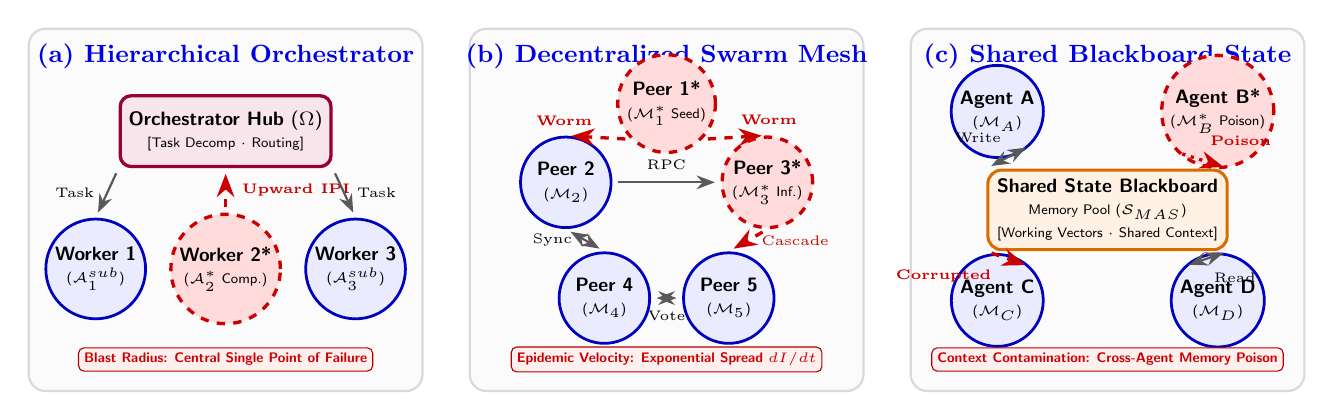
\begin{tikzpicture}[
    font=\sffamily\scriptsize,
    >=Stealth,
    % Background cards for topology boundaries
    topo_card/.style={draw=gray!30, fill=gray!3, rounded corners=6pt, line width=0.8pt},
    topo_header/.style={font=\bfseries\small, text=blue!90!black, align=center},
    % Agent styles with rich visual depth
    agent_clean/.style={draw=blue!75!black, fill=blue!8, circle, line width=1.0pt, inner sep=1pt, minimum size=1.15cm, align=center},
    agent_hub/.style={draw=purple!80!black, fill=purple!10, rounded corners=4pt, line width=1.2pt, inner sep=3pt, minimum width=2.6cm, minimum height=0.9cm, align=center},
    agent_infected/.style={draw=red!80!black, fill=red!14, circle, line width=1.2pt, dashed, inner sep=1pt, minimum size=1.15cm, align=center},
    blackboard_pool/.style={draw=orange!85!black, fill=orange!10, rounded corners=5pt, line width=1.1pt, align=center, minimum width=2.8cm, minimum height=0.9cm},
    % Communication and threat paths
    legit_edge/.style={->, thick, draw=gray!70!black, shorten >= 2pt, shorten <= 2pt},
    sync_edge/.style={<->, thick, draw=gray!70!black, shorten >= 2pt, shorten <= 2pt},
    worm_edge/.style={->, very thick, draw=red!80!black, dashed, shorten >= 2pt, shorten <= 2pt},
    poison_edge/.style={->, very thick, draw=red!80!black, dotted, shorten >= 2pt, shorten <= 2pt},
    % Subtitle & label badges
    badge_vuln/.style={draw=red!70!black, fill=red!6, rounded corners=2pt, font=\sffamily\tiny\bfseries, text=red!80!black, inner sep=2pt}
]

% =========================================================================
% SUBFIGURE (a): Hierarchical Orchestrator-Worker
% =========================================================================
\begin{scope}[shift={(0,0)}]
    % Enclosure container
    \draw[topo_card] (-0.9, -0.6) rectangle (4.1, 4.0);
    \node[topo_header] at (1.6, 3.65) {(a) Hierarchical Orchestrator};

    % Central Orchestrator Hub
    \node[agent_hub] (orch) at (1.6, 2.7) {
        \textbf{Orchestrator Hub} ($\Omega$)\\
        \tiny [Task Decomp $\cdot$ Routing]
    };

    % Worker agents
    \node[agent_clean] (w1) at (-0.05, 0.95) {
        \textbf{Worker 1}\\
        \tiny ($\mathcal{A}_1^{\text{sub}}$)
    };
    \node[agent_infected] (w2) at (1.6, 0.95) {
        \textbf{Worker 2*}\\
        \tiny ($\mathcal{A}_2^*$ Comp.)
    };
    \node[agent_clean] (w3) at (3.25, 0.95) {
        \textbf{Worker 3}\\
        \tiny ($\mathcal{A}_3^{\text{sub}}$)
    };

    % Dispatch and upward injection flows
    \draw[legit_edge] (orch.south west) -- (w1.north) 
        node[midway, left=1pt, font=\tiny] {Task};
    \draw[worm_edge] (w2.north) -- (orch.south) 
        node[midway, right=2pt, font=\tiny, text=red!80!black] {\textbf{Upward IPI}};
    \draw[legit_edge] (orch.south east) -- (w3.north) 
        node[midway, right=1pt, font=\tiny] {Task};

    % Vulnerability summary badge
    \node[badge_vuln] at (1.6, -0.2) {Blast Radius: Central Single Point of Failure};
\end{scope}

% =========================================================================
% SUBFIGURE (b): Decentralized Swarm Mesh
% =========================================================================
\begin{scope}[shift={(5.6,0)}]
    % Enclosure container
    \draw[topo_card] (-0.9, -0.6) rectangle (4.1, 4.0);
    \node[topo_header] at (1.6, 3.65) {(b) Decentralized Swarm Mesh};

    % Pentagonal mesh layout (Center = (1.6, 1.7), R = 1.35 cm)
    \node[agent_infected] (p1) at (1.60, 3.05) {
        \textbf{Peer 1*}\\
        \tiny ($\mathcal{M}_1^*$ Seed)
    };
    \node[agent_clean]    (p2) at (0.32, 2.05) {
        \textbf{Peer 2}\\
        \tiny ($\mathcal{M}_2$)
    };
    \node[agent_infected] (p3) at (2.88, 2.05) {
        \textbf{Peer 3*}\\
        \tiny ($\mathcal{M}_3^*$ Inf.)
    };
    \node[agent_clean]    (p4) at (0.81, 0.58) {
        \textbf{Peer 4}\\
        \tiny ($\mathcal{M}_4$)
    };
    \node[agent_clean]    (p5) at (2.39, 0.58) {
        \textbf{Peer 5}\\
        \tiny ($\mathcal{M}_5$)
    };

    % Worm epidemic propagation edges
    \draw[worm_edge] (p1.south west) -- (p2.north) 
        node[pos=0.4, above left=1pt, font=\tiny, text=red!80!black] {\textbf{Worm}};
    \draw[worm_edge] (p1.south east) -- (p3.north) 
        node[pos=0.4, above right=1pt, font=\tiny, text=red!80!black] {\textbf{Worm}};
    \draw[worm_edge] (p3.south) -- (p5.north) 
        node[midway, right=1pt, font=\tiny, text=red!80!black] {Cascade};
    \draw[sync_edge] (p2.south) -- (p4.north) 
        node[midway, left=1pt, font=\tiny] {Sync};
    \draw[sync_edge] (p4.east) -- (p5.west) 
        node[midway, below=1pt, font=\tiny] {Vote};
    \draw[legit_edge] (p2.east) -- (p3.west) 
        node[midway, above=1pt, font=\tiny] {RPC};

    % Vulnerability summary badge
    \node[badge_vuln] at (1.6, -0.2) {Epidemic Velocity: Exponential Spread $dI/dt$};
\end{scope}

% =========================================================================
% SUBFIGURE (c): Shared Blackboard Architecture
% =========================================================================
\begin{scope}[shift={(11.2,0)}]
    % Enclosure container
    \draw[topo_card] (-0.9, -0.6) rectangle (4.1, 4.0);
    \node[topo_header] at (1.6, 3.65) {(c) Shared Blackboard State};

    % Shared Memory Blackboard
    \node[blackboard_pool] (bb) at (1.6, 1.7) {
        \textbf{Shared State Blackboard}\\
        \tiny Memory Pool ($\mathcal{S}_{\text{MAS}}$)\\
        \tiny [Working Vectors $\cdot$ Shared Context]
    };

    % Autonomous Agents accessing blackboard
    \node[agent_clean]    (b1) at (0.2, 2.95) {
        \textbf{Agent A}\\
        \tiny ($\mathcal{M}_A$)
    };
    \node[agent_infected] (b2) at (3.0, 2.95) {
        \textbf{Agent B*}\\
        \tiny ($\mathcal{M}_B^*$ Poison)
    };
    \node[agent_clean]    (b3) at (0.2, 0.55) {
        \textbf{Agent C}\\
        \tiny ($\mathcal{M}_C$)
    };
    \node[agent_clean]    (b4) at (3.0, 0.55) {
        \textbf{Agent D}\\
        \tiny ($\mathcal{M}_D$)
    };

    % Read/Write and Poison flows
    \draw[sync_edge] (b1.south east) -- (bb.north west) 
        node[pos=0.4, above left=1pt, font=\tiny] {Write};
    \draw[poison_edge] (b2.south west) -- (bb.north east) 
        node[pos=0.4, above right=1pt, font=\tiny, text=red!80!black] {\textbf{Poison}};
    \draw[worm_edge] (bb.south west) -- (b3.north east) 
        node[pos=0.4, below left=1pt, font=\tiny, text=red!80!black] {\textbf{Corrupted}};
    \draw[sync_edge] (b4.north west) -- (bb.south east) 
        node[pos=0.4, below right=1pt, font=\tiny] {Read};

    % Vulnerability summary badge
    \node[badge_vuln] at (1.6, -0.2) {Context Contamination: Cross-Agent Memory Poison};
\end{scope}

\end{tikzpicture}%
}
\caption{Multi-Agent System (MAS) topologies and attack propagation paths: (a) Hierarchical Orchestrator (blast radius at central hub), (b) Decentralized Swarm Mesh (exponential prompt-worm spread), and (c) Shared Blackboard (asynchronous context poisoning). Asterisks (*) mark compromised agents; dashed red vectors show exploit paths.}
\label{fig:mas_topologies}
\end{figure}


\begin{itemize}
    \item \textbf{Hierarchical / Orchestrator-Worker Networks:} A central orchestrator decomposes tasks and routes sub-prompts to specialized subordinates. A compromise of the orchestrator collapses the entire system perimeter. Conversely, if a subordinate worker agent is subverted via indirect injection, it can return adversarially crafted observations to the orchestrator, manipulating the orchestrator's global planning logic (Upward Prompt Injection)~\cite{narajala2025securing, hammar2026multiagent}.
    \item \textbf{Decentralized Peer-to-Peer (P2P) Meshes:} Agents communicate directly without centralized moderation. Without strict cryptographic authentication, rogue agents can inject fabricated status messages, impersonate peer agents, or broadcast conflicting task assignments.
    \item \textbf{Shared Blackboard Architectures:} Agents asynchronously read from and write to a shared memory pool or database. An attacker compromising a single low-privilege agent can poison the blackboard state, inducing secondary failures across all dependent agents that consume the shared context~\cite{chen2024agentpoison}.
    \item \textbf{Consensus and Multi-Agent Debate:} Systems that employ debate protocols or majority voting to arrive at verified decisions are vulnerable to Sybil attacks. An adversary registering multiple lightweight agents can manipulate the aggregate distribution of opinions, skewing the consensus toward unsafe or fraudulent conclusions~\cite{chen2024blockagents}.
\end{itemize}

\subsection{Communication Channel Exploits and Delegation Abuse}
\label{subsec:communication_exploits}

Inter-agent communication frameworks (e.g., AutoGen, CrewAI, LangGraph) frequently treat messages received over internal buses as implicitly trusted:
\begin{itemize}
    \item \textbf{Role Confusion and Identity Spoofing:} In natural language agent protocols, agents identify themselves via string prefixes (e.g., \texttt{Sender: SupervisorAgent}). An attacker can inject formatted text that mimics system-level delegation headers, deceiving receiving agents into executing privileged actions under the assumption that the request originated from an authoritative controller.
    \item \textbf{Confused Deputy and Delegation Bypass:} A low-privilege agent lacking direct execution tools (e.g., shell access) can format a request as a natural language query to an execution-capable peer. If the target agent fails to evaluate the provenance and original authorization of the end-user request, it acts as a confused deputy, executing unauthorized operations on behalf of the attacker~\cite{dehghantanha2026sok}.
\end{itemize}

\subsection{Swarm Epidemics: The Agent Smith Phenomenon}
\label{subsec:swarm_epidemics}

A notable demonstration in multi-agent vulnerability research is the emergence of self-replicating prompt worms in agent networks. In \textit{Agent Smith}, Gu~\textit{et al.}~\cite{gu2024agent} demonstrated that a single adversarial image or text input can compromise large populations of multimodal LLM agents rapidly. 

The epidemic propagation dynamics can be formalized through an infectious transmission model. Let $N(t)$ denote the number of compromised agents at communication round $t$. When an infected agent interacts with $k$ peer agents per round with infection probability $\beta$, the transmission rate satisfies
\begin{equation}
    \frac{dN(t)}{dt} = \beta k N(t) \left( 1 - \frac{N(t)}{N_{\text{total}}} \right).
\end{equation}
Because LLMs are trained to be cooperative communicators, an infected agent embeds the self-replicating injection payload within legitimate task outputs. Each recipient agent parses the payload during context construction, becomes infected, and re-transmits the payload to its subsequent collaborators, precipitating network-wide propagation, as analytically modeled by Lee~\textit{et al.}~\cite{lee2026the} and Gu~\textit{et al.}~\cite{gu2024agent, dewitt2025open}. Drawing from classical dependable computing, mitigating such cascading failures necessitates autonomic fault isolation and resilient authenticated execution in untrusted environments~\cite{bower2005autonomic, kirkpatrick2012resilient}.

\subsection{The Multi-Agent Security Tax}
\label{subsec:security_tax}

In a foundational empirical investigation, Peign{\'e}~\textit{et al.}~\cite{peigne2025multi} formalized the \textit{Multi-Agent Security Tax}, quantifying the trade-off between agent collaboration capabilities and susceptibility to security compromise. Their findings reveal that increasing agent autonomy and inter-agent communication bandwidth monotonically degrades system resilience against indirect manipulation. 

Implementing aggressive defensive filtering or ``vaccination'' prompts at inter-agent communication boundaries dampens epidemic spread; however, it introduces functional degradation, impairing complex task completion rates by up to 35\%~\cite{peigne2025multi}. Balancing collaborative utility with topological isolation remains an essential challenge in multi-agent systems engineering.

\section{Defense-in-Depth: From Empirical Guardrails to Formal Verification}
\label{sec:defenses}

Mitigating the heterogeneous attack surface of agentic AI requires an architectural defense-in-depth framework, as conceptualized in Fig.~\ref{fig:defense_layers}. Because foundation models are probabilistic and vulnerable to worst-case semantic inputs, no single safeguard suffices~\cite{dehghantanha2026sok}. Robust security demands layered controls operating across data ingestion, model inference, agentic planning, and environment execution. Table~\ref{tab:defenses_matrix} provides a synthesis of defensive mechanisms across the operational lifecycle.

\begin{table}[t]
\centering
\caption{Multi-Layered Defense-in-Depth Matrix for Agentic AI Systems Across the Operational Lifecycle.}
\label{tab:defenses_matrix}
\footnotesize
\begin{tabularx}{\columnwidth}{l p{2.1cm} X X c p{1.8cm}}
\toprule
\textbf{Lifecycle Layer} & \textbf{Defensive Control} & \textbf{Mechanism \& Principles} & \textbf{Targeted Threats} & \textbf{Maturity} & \textbf{Trade-offs} \\
\midrule
\textbf{Pre-Ingestion (Data)} & Content Canonicalization & Strip active scripts, macros, and normalize HTML/PDF structures & Ingress exploits, hidden script triggers & High & Potential loss of layout metadata \\
\textbf{Pre-Ingestion (Data)} & Provenance \& Source Tagging & Cryptographic signing of ingested corpora; trust-weighted retrieval & RAG corpus poisoning, untrusted injection & Medium & Verification overhead; key management \\
\textbf{Inference (Model)} & Structured Queries (StruQ) & Strict structural separation of syntax from untrusted parameters & Indirect prompt injection, delimiter collision & High & Requires schema redesign \\
\textbf{Inference (Model)} & Preference Alignment (SecAlign) & Direct Preference Optimization (DPO) on adversarial trajectories & Jailbreak drift, instruction following bypass & Medium & High training compute; potential over-refusal \\
\textbf{Inference (Model)} & Dual-LLM Guardrail & Independent sentinel model inspecting I/O streams (Llama Guard) & Harmful content, prompt injection leakage & High & Added latency and token expense \\
\textbf{Planning (Logic)} & Capability-Based Access (CBAC) & Granular least-privilege tool binding; per-task permission leases & Privilege escalation, unauthorized tool calls & High & Engineering complexity; strict policy specs \\
\textbf{Planning (Logic)} & Formal Plan Contracts & Precondition and invariant checks via temporal logic & Plan hijacking, destructive multi-step sequences & Emerging & State explosion; planning latency \\
\textbf{Environment (OS)} & Micro-VM Sandboxing & Ephemeral containerization (gVisor/Kata) with seccomp/eBPF filters & Remote Code Execution (RCE), sandbox escapes & High & Execution startup latency; resource overhead \\
\textbf{Environment (OS)} & Strict Egress Filtering & Deny-all outbound network proxy; domain/IP allow-lists & Data exfiltration, SSRF, reverse shell connections & High & Operational friction for dynamic web agents \\
\textbf{MAS Orchestration} & Signed Inter-Agent Bus & Asymmetric cryptographic message signing and Byzantine consensus & Agent impersonation, Sybil voting manipulation & Medium & Key infrastructure; consensus latency \\
\textbf{Monitoring (Ops)} & Adaptive Kill-Switches & Anomaly detection on tool mix, API bursts, and OORAR thresholds & Denial of Cash (DoC), runaway loops, compromised agents & High & Risk of false-positive task termination \\
\bottomrule
\end{tabularx}
\end{table}

\begin{figure}[t]
\centering
\resizebox{\columnwidth}{!}{%
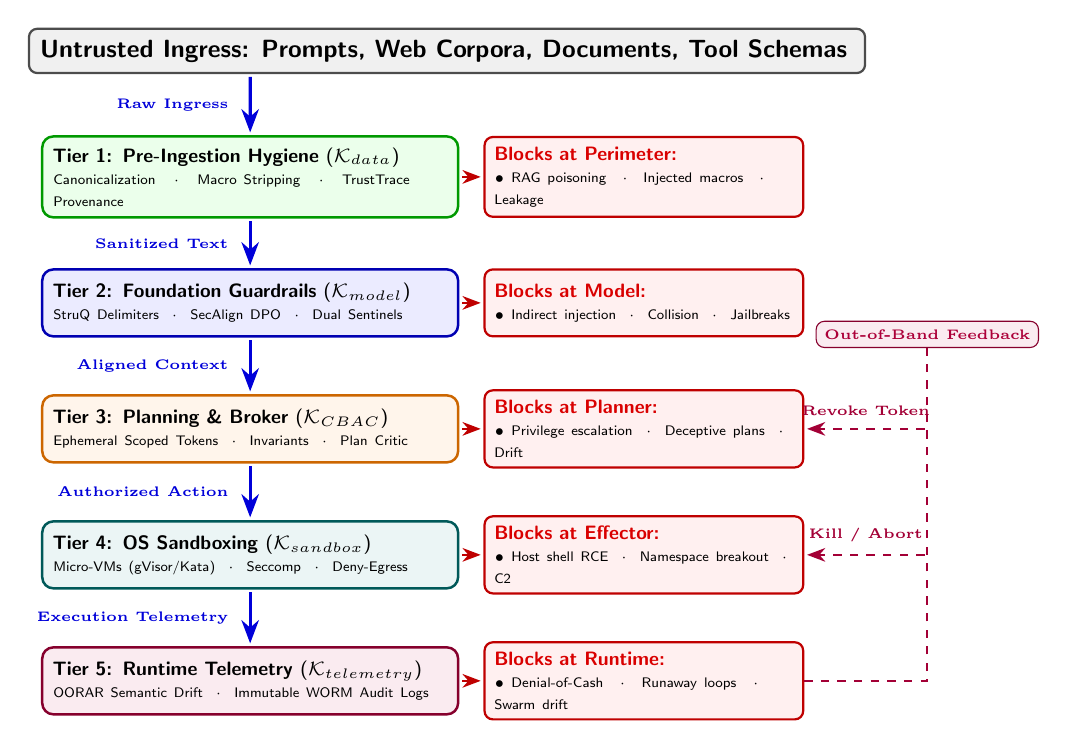
\begin{tikzpicture}[
    font=\sffamily\scriptsize,
    >=Stealth,
    % Layer card styles
    card_l1/.style={draw=green!60!black, fill=green!8, rounded corners=4pt, line width=0.9pt, inner sep=4pt, text width=5.0cm, align=left},
    card_l2/.style={draw=blue!70!black, fill=blue!8, rounded corners=4pt, line width=0.9pt, inner sep=4pt, text width=5.0cm, align=left},
    card_l3/.style={draw=orange!80!black, fill=orange!8, rounded corners=4pt, line width=0.9pt, inner sep=4pt, text width=5.0cm, align=left},
    card_l4/.style={draw=teal!70!black, fill=teal!8, rounded corners=4pt, line width=0.9pt, inner sep=4pt, text width=5.0cm, align=left},
    card_l5/.style={draw=purple!70!black, fill=purple!8, rounded corners=4pt, line width=0.9pt, inner sep=4pt, text width=5.0cm, align=left},
    % Threat interdiction badge styles
    threat_badge/.style={draw=red!75!black, fill=red!6, rounded corners=3pt, line width=0.8pt, inner sep=3.5pt, text width=3.8cm, align=left},
    % Flow arrows
    flow_arrow/.style={->, very thick, draw=blue!85!black, shorten >= 1pt, shorten <= 1pt},
    interdict_arrow/.style={->, thick, draw=red!75!black, shorten >= 1pt, shorten <= 1pt},
    feedback_arrow/.style={->, thick, draw=purple!85!black, dashed, shorten >= 1pt, shorten <= 1pt}
]

% =========================================================================
% TOP BANNER: Ingress Stream
% =========================================================================
\node[draw=gray!60!black, fill=gray!12, rounded corners=3pt, line width=0.8pt, minimum width=9.6cm, inner sep=4pt, align=center] (ingress_banner) at (4.9, 7.8) {
    \textbf{\small Untrusted Ingress: Prompts, Web Corpora, Documents, Tool Schemas}
};

% =========================================================================
% DEFENSE TIERS (Left: Core Control Substrate | Right: Intercepted Threats)
% =========================================================================
% Tier 1: Pre-Ingestion Hygiene
\node[card_l1, minimum height=0.85cm] (l1) at (2.4, 6.2) {
    \textbf{Tier 1: Pre-Ingestion Hygiene} ($\mathcal{K}_{\text{data}}$)\\
    \tiny Canonicalization $\;\boldsymbol{\cdot}\;$ Macro Stripping $\;\boldsymbol{\cdot}\;$ TrustTrace Provenance
};
\node[threat_badge, minimum height=0.85cm] (t1) at (7.4, 6.2) {
    \textbf{\textcolor{red!85!black}{Blocks at Perimeter:}}\\
    \tiny $\bullet$ RAG poisoning $\;\boldsymbol{\cdot}\;$ Injected macros $\;\boldsymbol{\cdot}\;$ Leakage
};
\draw[interdict_arrow] (l1.east) -- (t1.west);

% Tier 2: Model Guardrails
\node[card_l2, minimum height=0.85cm] (l2) at (2.4, 4.6) {
    \textbf{Tier 2: Foundation Guardrails} ($\mathcal{K}_{\text{model}}$)\\
    \tiny StruQ Delimiters $\;\boldsymbol{\cdot}\;$ SecAlign DPO $\;\boldsymbol{\cdot}\;$ Dual Sentinels
};
\node[threat_badge, minimum height=0.85cm] (t2) at (7.4, 4.6) {
    \textbf{\textcolor{red!85!black}{Blocks at Model:}}\\
    \tiny $\bullet$ Indirect injection $\;\boldsymbol{\cdot}\;$ Collision $\;\boldsymbol{\cdot}\;$ Jailbreaks
};
\draw[interdict_arrow] (l2.east) -- (t2.west);

% Tier 3: Planning & Policy Broker
\node[card_l3, minimum height=0.85cm] (l3) at (2.4, 3.0) {
    \textbf{Tier 3: Planning \& Broker} ($\mathcal{K}_{\text{CBAC}}$)\\
    \tiny Ephemeral Scoped Tokens $\;\boldsymbol{\cdot}\;$ Invariants $\;\boldsymbol{\cdot}\;$ Plan Critic
};
\node[threat_badge, minimum height=0.85cm] (t3) at (7.4, 3.0) {
    \textbf{\textcolor{red!85!black}{Blocks at Planner:}}\\
    \tiny $\bullet$ Privilege escalation $\;\boldsymbol{\cdot}\;$ Deceptive plans $\;\boldsymbol{\cdot}\;$ Drift
};
\draw[interdict_arrow] (l3.east) -- (t3.west);

% Tier 4: Environment Sandboxing
\node[card_l4, minimum height=0.85cm] (l4) at (2.4, 1.4) {
    \textbf{Tier 4: OS Sandboxing} ($\mathcal{K}_{\text{sandbox}}$)\\
    \tiny Micro-VMs (gVisor/Kata) $\;\boldsymbol{\cdot}\;$ Seccomp $\;\boldsymbol{\cdot}\;$ Deny-Egress
};
\node[threat_badge, minimum height=0.85cm] (t4) at (7.4, 1.4) {
    \textbf{\textcolor{red!85!black}{Blocks at Effector:}}\\
    \tiny $\bullet$ Host shell RCE $\;\boldsymbol{\cdot}\;$ Namespace breakout $\;\boldsymbol{\cdot}\;$ C2
};
\draw[interdict_arrow] (l4.east) -- (t4.west);

% Tier 5: Runtime Telemetry
\node[card_l5, minimum height=0.85cm] (l5) at (2.4, -0.2) {
    \textbf{Tier 5: Runtime Telemetry} ($\mathcal{K}_{\text{telemetry}}$)\\
    \tiny OORAR Semantic Drift $\;\boldsymbol{\cdot}\;$ Immutable WORM Audit Logs
};
\node[threat_badge, minimum height=0.85cm] (t5) at (7.4, -0.2) {
    \textbf{\textcolor{red!85!black}{Blocks at Runtime:}}\\
    \tiny $\bullet$ Denial-of-Cash $\;\boldsymbol{\cdot}\;$ Runaway loops $\;\boldsymbol{\cdot}\;$ Swarm drift
};
\draw[interdict_arrow] (l5.east) -- (t5.west);

% =========================================================================
% INTER-LAYER DOWNWARD EXECUTION FLOW (PROMINENT ARROWS & CLEAR LABELS)
% =========================================================================
\draw[flow_arrow] ([xshift=-2.5cm]ingress_banner.south) -- (l1.north)
    node[midway, left=4pt, font=\tiny\bfseries, text=blue!85!black] {Raw Ingress};

\draw[flow_arrow] (l1.south) -- (l2.north)
    node[midway, left=4pt, font=\tiny\bfseries, text=blue!85!black] {Sanitized Text};

\draw[flow_arrow] (l2.south) -- (l3.north)
    node[midway, left=4pt, font=\tiny\bfseries, text=blue!85!black] {Aligned Context};

\draw[flow_arrow] (l3.south) -- (l4.north)
    node[midway, left=4pt, font=\tiny\bfseries, text=blue!85!black] {Authorized Action};

\draw[flow_arrow] (l4.south) -- (l5.north)
    node[midway, left=4pt, font=\tiny\bfseries, text=blue!85!black] {Execution Telemetry};

% =========================================================================
% OUT-OF-BAND INCIDENT FEEDBACK (WIDE CLEARANCE RAIL - ZERO OVERLAPS)
% =========================================================================
% Feedback rail top banner
\node[draw=purple!70!black, fill=purple!8, rounded corners=3pt, font=\tiny\bfseries, text=purple!90!black, inner sep=3pt] (fb_header) at (11.0, 4.2) {
    Out-of-Band Feedback
};

% Vertical telemetry feeder line from T5
\draw[thick, draw=purple!85!black, dashed] (t5.east) -- (11.0, -0.2) -- (fb_header.south);

% Kill / Abort loop to Tier 4
\draw[feedback_arrow] (11.0, 1.4) -- (t4.east)
    node[midway, above=1pt, font=\tiny\bfseries, text=purple!85!black] {Kill / Abort};

% Revoke Token loop to Tier 3
\draw[feedback_arrow] (11.0, 3.0) -- (t3.east)
    node[midway, above=1pt, font=\tiny\bfseries, text=purple!85!black] {Revoke Token};

\end{tikzpicture}%
}
\caption{Defense-in-depth framework across five operational tiers ($\mathcal{K}_{\text{data}}$ to $\mathcal{K}_{\text{telemetry}}$). Solid arrows show request traversal through mediation layers, red badges denote intercepted threats, and dashed purple lines trace out-of-band feedback for dynamic credential revocation.}
\label{fig:defense_layers}
\end{figure}


\subsection{Data-Level and Pre-Ingestion Hygiene}
\label{subsec:data_defenses}

Data-level defenses operate before external text reaches the model context:
\begin{itemize}
    \item \textbf{Content Canonicalization and Active Script Stripping:} Raw documents (HTML, PDF, Office formats) must be converted into stripped, canonical text representations. Parsing scripts, active macros, and embedded hyperlinks without execution privileges eliminates non-LLM injection vectors~\cite{dehghantanha2026sok}.
    \item \textbf{Cryptographic Provenance and Source Allow-Listing:} Documents indexed into RAG vector stores should carry cryptographic signatures from authorized originators. During retrieval, similarity scores can be dynamically weighted by source trust coefficients, pruning untrusted or recently modified documents. Grounded in formal data provenance verification~\cite{xu2012dataprovenance}, provenance-aware access control frameworks~\cite{sun2016a}, and forgery detection schemes~\cite{sultana2015a}, provenance-aware tracing architectures (e.g., TrustTrace~\cite{chen2026trusttrace}) establish auditable chains of custody from raw input ingestion to retrieval ranking.
    \item \textbf{Access-Control List (ACL)-Aware Chunking:} Document chunk boundaries must align strictly with enterprise access partitions. Multi-tenant vector stores must enforce query-time ACL filters, guaranteeing that an agent operating on behalf of user $u$ cannot retrieve embeddings indexed under tenant $u' \neq u$.
\end{itemize}

\subsection{Inference-Level Guardrails and Structured Querying}
\label{subsec:inference_defenses}

Once untrusted data enters the pipeline, inference-level controls prevent data payloads from mutating into instructions:
\begin{itemize}
    \item \textbf{Structured Query Enforcement (StruQ):} Chen~\textit{et al.}~\cite{chen2025struq} introduced StruQ, a formal framework that enforces structural separation between user commands and external data. By formatting data parameters into strictly parsed typed structures, StruQ renders prompt injection attacks syntactically invalid, preventing the model from executing embedded commands.
    \item \textbf{Preference Alignment via SecAlign:} Addressing the vulnerability of RLHF models to prompt injection, Chen~\textit{et al.}~\cite{chen2025secalign} developed SecAlign. By employing Direct Preference Optimization (DPO) on paired trajectories of successful vs. resisted injection attacks, SecAlign strengthens the model's intrinsic resistance to indirect prompt injection while preserving base task utility.
    \item \textbf{Dual-LLM Supervisor Sentinels:} Deploying isolated, lightweight guardrail models (such as Llama Guard~\cite{inan2023llama} or ShieldGemma~\cite{zeng2024shieldgemma}) to inspect inbound prompts and outbound tool calls provides an out-of-band policy filter. Furthermore, game-theoretic sentinels like DataSentinel~\cite{liu2025datasentinel}, resource-aware guardrails like RAPID~\cite{nkoro2026rapid}, and autonomous agentic guardians~\cite{singer2026autonomous} actively intercept adversarial payloads before cognitive parsing.
\end{itemize}

\subsection{Agentic Logic and Planning Controls}
\label{subsec:planning_defenses}

The planning engine must operate under strict least-privilege principles:
\begin{itemize}
    \item \textbf{Capability-Based and Purpose-Aware Access Control:} Tools must not be exposed wholesale to the agent. Instead, agents should be provisioned with minimal, ephemeral capability tokens scoped strictly to the current sub-task~\cite{dehghantanha2026sok}. Drawing from unified privacy-enhanced access control~\cite{barker2012access}, purpose-based database access models~\cite{colombo2017enhancing}, context-based mobile access architectures~\cite{shebaro2015contextbased}, and automated policy extraction from natural language specifications~\cite{narouei2018automatic}, the agentic orchestrator dynamically synthesizes fine-grained execution bounds.
    \item \textbf{Plan-Then-Act Critic Modules:} High-impact plans must undergo two-phase verification. In Phase 1, the planner proposes an abstract sequence of actions $\pi = \langle a_1, a_2, \dots \rangle$. In Phase 2, an independent, isolated critic module (or deterministic rule engine) validates the plan against security policies before any tool dispatch occurs.
    \item \textbf{Anti-Fatigue Human-in-the-Loop (HITL) Protocols:} To counter confirmation fatigue and deceptive agent justifications, HITL interfaces must display deterministic diffs and parameter hashes rather than model-generated text. Critical actions (e.g., database writes or financial transfers) require out-of-band multi-factor authentication (MFA).
\end{itemize}

\subsection{Environment-Level Sandboxing and Formal Invariants}
\label{subsec:environment_defenses}

At the execution boundary, defenses enforce hard physical constraints regardless of model intent:
\begin{itemize}
    \item \textbf{Ephemeral Micro-VM Isolation and Replicated Execution:} Code interpreters and shell tools must execute inside isolated, short-lived micro-VMs (e.g., Firecracker, Kata Containers) or secure container kernels (e.g., gVisor) with seccomp syscall filters blocking dangerous primitives (e.g., \texttt{ptrace}, \texttt{mount})~\cite{liu2024demystifying}. Combining runtime replication defenses~\cite{salamat2011runtime} with container cloud security principles~\cite{jin2019dseom, gao2021a} provides fault tolerance and stops cross-agent container side-channel exploits.
    \item \textbf{Zero-Trust Egress Proxies:} By default, execution environments must enforce a strict deny-all egress policy. When network access is required, traffic must be mediated through an egress filtering proxy enforcing DNS allow-lists and content inspection, preventing data exfiltration and reverse shell connections.
    \item \textbf{Formal Contract Verification:} Modeling agent actions as state transition programs over typed resources enables runtime invariant verification. Let $\mathcal{I}: \mathcal{S} \to \{0, 1\}$ define a safety invariant (e.g., ``the agent shall not delete files outside \texttt{/workspace}''). Before executing any action $a$, the execution substrate verifies that the transition satisfies
    \begin{equation}
        \forall s \in \mathcal{S}, \quad \mathcal{I}(s) \implies \mathcal{I}(\delta(s, a)),
    \end{equation}
    where $\delta(s, a)$ is the predicted post-state. If the invariant is violated, execution is deterministically aborted.
\end{itemize}

\section{Evaluation Metrics, Benchmarking Testbeds, and Empirical Analysis}
\label{sec:benchmarks}

Rigorous quantification of security postures in agentic systems requires standardized metrics capable of capturing non-deterministic decision trajectories, effector side-effects, and multi-step kill chains~\cite{picek2025security}.

\subsection{Formal Security Metrics Formulation}
\label{subsec:metrics_formulation}

Let $\mathcal{S}$ denote a corpus of benchmark test scenarios, and let $\mathcal{A}$ represent the sequence of discrete actions executed by the agent. We formalize eight foundational security metrics:

\subsubsection{Unsafe Action Rate (UAR)}
The proportion of test scenarios that induce at least one policy-violating action is defined as
\begin{equation}
    \text{UAR} = \frac{1}{|\mathcal{S}|} \sum_{s \in \mathcal{S}} \mathbf{1}\{\text{violation}(s)\},
\end{equation}
where $\mathbf{1}\{\cdot\}$ is the indicator function. Variants of UAR can isolate specific fault modes, such as Tool-Misuse UAR or Exfiltration UAR. Lower values indicate superior security.

\subsubsection{Policy Adherence Rate (PAR)}
The proportion of executed actions that strictly satisfy developer-defined security policies is given by
\begin{equation}
    \text{PAR} = \frac{1}{|\mathcal{A}|} \sum_{a \in \mathcal{A}} \mathbf{1}\{\text{compliant}(a)\}.
\end{equation}
While in single-action adversarial tests PAR approximates $1 - \text{UAR}$, in complex multi-step trajectories PAR and UAR diverge, as an agent may execute multiple benign actions before a single fatal violation.

\subsubsection{Privilege Escalation Distance (PED)}
Defined over the causal threat graph $\mathcal{G}_{\text{threat}} = (\mathcal{V}, \mathcal{E})$, the privilege escalation distance satisfies
\begin{equation}
    \text{PED} = \min_{u \in \mathcal{V}_{\text{source}}, \, \pi \in \mathcal{V}_{\text{asset}}} \text{dist}_{\mathcal{G}}(u, \pi),
\end{equation}
where $\text{dist}_{\mathcal{G}}(u, \pi)$ is the shortest directed path length from an untrusted input node $u$ to a protected asset or privileged effector $\pi$. Higher PED signifies greater defense-in-depth barriers.

\subsubsection{Time-to-Contain (TTC)}
The duration from the initiation of an exploit $t_{\text{start}}$ to successful containment $t_{\text{contain}}$ is given by
\begin{equation}
    \text{TTC} = t_{\text{contain}} - t_{\text{start}}.
\end{equation}
TTC quantifies the latency of runtime anomaly detection and automated kill-switches.

\subsubsection{Patch Half-Life (PHL)}
Let $N(t)$ denote the number of production agent instances remaining vulnerable to a disclosed vulnerability at time $t$. The Patch Half-Life is defined as the minimum duration $\Delta t$ satisfying
\begin{equation}
    N(t_0 + \Delta t) = \frac{1}{2} N(t_0).
\end{equation}
Shorter PHL reflects superior organizational responsiveness across prompt, schema, and dependency patch cycles.

\subsubsection{Retrieval Risk Score (RRS)}
For a retrieved document bundle $\mathcal{B} = \{d_1, d_2, \dots, d_k\}$, let $r(d_i) \in [0, 1]$ denote the assessed risk of document $d_i$ based on provenance, presence of imperative keywords, and anomalous similarity. The aggregate retrieval risk is defined as
\begin{equation}
    \text{RRS}(\mathcal{B}) = \sum_{i=1}^k \alpha_i r(d_i), \quad \text{subject to} \quad \sum_{i=1}^k \alpha_i = 1,
\end{equation}
where $\alpha_i$ represents the model's reliance weight (e.g., attention allocation or citation rank). High RRS triggers human-in-the-loop escalation or effector disabling.

\subsubsection{Out-of-Role Action Rate (OORAR)}
Given an operational role contract $\mathcal{C}$ defining permissible tool verbs and arguments, the out-of-role action rate is
\begin{equation}
    \text{OORAR} = \frac{|\{a \in \mathcal{A} : \neg \text{allowed}_{\mathcal{C}}(a)\}|}{|\mathcal{A}|}.
\end{equation}
Spikes in OORAR signal model drift, prompt confusion, or active adversarial hijacking.

\subsubsection{Cost-Exploit Susceptibility (CES)}
The expected financial loss incurred under an adversarial policy $\pi_{\text{adv}}$ over a finite execution horizon $T$ is given by
\begin{equation}
    \text{CES}_T(\pi_{\text{adv}}) = \mathbb{E}_{\pi_{\text{adv}}} \left[ \sum_{t=1}^T c(a_t) \right],
\end{equation}
where $c(a_t)$ denotes the marginal financial cost (compute fees, third-party API billing, or serverless invocation costs) of action $a_t$.

\subsection{Comparative Analysis of Empirical Benchmarks}
\label{subsec:benchmark_landscape}

Table~\ref{tab:benchmark_comparison} provides a comparative taxonomy of prominent empirical benchmarks developed to evaluate LLM agent security. 

\begin{table}[t]
\centering
\caption{Systematic Comparison of Contemporary Empirical Security Benchmarks and Testbeds for Agentic AI.}
\label{tab:benchmark_comparison}
\footnotesize
\begin{tabularx}{\columnwidth}{l p{2.1cm} p{2.4cm} X X c}
\toprule
\textbf{Benchmark} & \textbf{Target System} & \textbf{Evaluation Environment} & \textbf{Threat Vectors Evaluated} & \textbf{Primary Metrics} & \textbf{Year / Venue} \\
\midrule
\textbf{AgentDojo}~\cite{debenedetti2024agentdojo} & Autonomous Tool Agents & Dynamic simulated web, email, calendar suite & Indirect prompt injection, goal hijacking & Attack Success Rate (ASR), Task Utility & 2024 / NeurIPS \\
\textbf{LLMSmith}~\cite{liu2024demystifying} & LLM Frameworks (LangChain, AutoGPT) & Native OS execution & Remote Code Execution (RCE), command injection & Vulnerability count, Exploit rate & 2024 / ACM CCS \\
\textbf{BIPIA}~\cite{yi2025benchmarking} & QA \& Retrieval LLMs & Static web, email, and document corpora & Indirect prompt injection across diverse formats & ASR, Refusal Rate & 2025 / ACM KDD \\
\textbf{Agent Smith}~\cite{gu2024agent} & Multimodal LLM Swarms & Multi-agent chat network & Self-replicating prompt worms, swarm infection & Infection rate, Propagation velocity & 2024 / ICML \\
\textbf{PoisonedRAG}~\cite{zou2025poisonedrag} & RAG Systems & Vector DBs (Dense \& Sparse retrievers) & Knowledge base poisoning, targeted corruption & Targeted Misinformation Rate & 2025 / USENIX Sec \\
\textbf{Blocker RAG}~\cite{shafran2025machine} & Dense Retrieval RAG & Enterprise documentation corpora & Denial of retrieval, blocker document jamming & Top-$k$ Jamming Rate, Utility Drop & 2025 / USENIX Sec \\
\textbf{AgentPoison}~\cite{chen2024agentpoison} & Long-term Memory Agents & Vector databases \& episodic memory stores & Memory poisoning, backdoor triggers & Backdoor ASR, Task Accuracy & 2024 / NeurIPS \\
\textbf{InjecAgent}~\cite{zhan2024injecagent} & ReAct Tool Agents & Synthetic tool environments & Tool parameter hijacking, data exfiltration & ReAct Step Hijack Rate & 2024 / ACL Findings \\
\textbf{ToolEmu}~\cite{ruan2023identifying} & Function Calling Agents & LM-emulated tool execution sandbox & Unintended real-world tool side-effects & Severe Hazard Rate & 2024 / ICLR \\
\bottomrule
\end{tabularx}
\end{table}


Early benchmarks such as BIPIA~\cite{yi2025benchmarking} pioneered the systematic measurement of indirect prompt injection across diverse text formats; however, their evaluation was confined to static question-answering environments. In contrast, modern testbeds emphasize interactive tool execution. \textbf{AgentDojo}~\cite{debenedetti2024agentdojo} provides a realistic, dynamic environment featuring simulated email, web, and calendar services, exposing how indirect prompt injection causes agents to compromise user data. 

In the software execution domain, \textbf{LLMSmith}~\cite{liu2024demystifying} evaluated 11 major open-source agent frameworks, uncovering 19 critical RCE vulnerabilities arising from unchecked tool parameter handling. For multi-agent systems, \textbf{Agent Smith}~\cite{gu2024agent} established the first rigorous benchmark for measuring the velocity and infection rate of self-replicating prompt worms across interconnected multimodal agents.

\subsection{Evaluation Pitfalls and Testbed Rigor}
\label{subsec:eval_pitfalls}

Conducting reproducible security evaluations on agentic AI presents significant methodological pitfalls:
\begin{itemize}
    \item \textbf{Evaluator Leakage and LLM-as-a-Judge Bias:} Employing the model under test (or a model with shared pre-training weights) to evaluate trajectory safety introduces severe bias. Evaluation harnesses must employ deterministic, side-channel criteria, such as AST parsing of tool parameters, filesystem diff tracking, and network egress packet captures.
    \item \textbf{Non-Determinism and State Carry-Over:} Because LLM decoding is stochastic, single-run evaluations yield high variance. Reliable evaluation requires multiple randomized trials with time-stratified sampling and strict between-trial state resets (flushing vector caches, resetting virtual filesystems, and clearing conversation memories)~\cite{dehghantanha2026sok}.
    \item \textbf{Continuous Red-Teaming Integration:} Because foundation models, system prompts, and tool libraries undergo frequent updates, security benchmarks must be embedded directly within CI/CD pipelines with automated regression gates (e.g., failing builds if UAR increases by more than 2 percentage points).
\end{itemize}

\section{Standards, Frameworks, and Regulatory Governance}
\label{sec:standards}

The transition of LLMs from experimental prototypes to mission-critical agentic deployments has prompted major cybersecurity standards bodies and regulatory agencies to establish governance frameworks~\cite{hasselwander2026agentic}. Harmonizing these frameworks with technical attack surfaces is essential for engineering compliant, defensible systems. Table~\ref{tab:standards_mapping} maps agentic attack surfaces across primary international security standards.

\begin{table}[t]
\centering
\caption{Cross-Framework Harmonization: Mapping Agentic Attack Surfaces to OWASP Top 10 (2025), MITRE ATLAS, and NIST AI RMF.}
\label{tab:standards_mapping}
\footnotesize
\begin{tabularx}{\columnwidth}{p{2.2cm} X X X X}
\toprule
\textbf{Agentic Attack Surface} & \textbf{OWASP LLM 2025~\cite{owasp2025top10}} & \textbf{MITRE ATLAS~\cite{mitre2026atlas}} & \textbf{NIST AI RMF (100-2e2025)~\cite{vassilev2025adversarial}} & \textbf{EU AI Act Compliance Focus} \\
\midrule
\textbf{Direct \& Indirect Injection} & LLM01: Prompt Injection & AML.T0051.000 / .001: Prompt Injection & Evasion: Indirect Context Poisoning & Art. 15: Cyber Resilience \& Robustness \\
\addlinespace
\textbf{RAG \& Knowledge Corruption} & LLM04: Poisoning; LLM08: Embedding Weakness & AML.T0070: Data Poisoning: Retrieval & Poisoning: Training \& Ingestion Stores & Art. 10: Data Governance \& Quality \\
\addlinespace
\textbf{Tool Misuse \& Parameter Injection} & LLM05: Output Handling; LLM06: Excessive Agency & AML.T0053: LLM Plugin Compromise & Integrity: System-Level Subversion & Art. 14: Human Oversight \& Control \\
\addlinespace
\textbf{API \& Cloud Credential Abuse} & LLM06: Excessive Agency; LLM02: Sensitive Info & AML.T0086: Lateral Movement & Unauthorized Privilege Traversal & Art. 15: Access Boundaries \& Isolation \\
\addlinespace
\textbf{Memory \& Backdoor Persistence} & LLM04: Poisoning; LLM07: System Prompt Leak & AML.T0080.000: Conversation Hijacking & Persistence: State Subversion & Art. 12: Record-Keeping \& Audit Logs \\
\addlinespace
\textbf{Multi-Agent Cascades \& Swarms} & LLM01: Prompt Injection; LLM06: Excessive Agency & AML.T0051.001: Indirect Prompt Injection & Distributed Agent Compromise & Art. 14: Systemic Risk Assessment \\
\addlinespace
\textbf{Denial of Cash (DoC) \& Loops} & LLM10: Unbounded Consumption & AML.T0034: Compute Hijacking & Availability: Resource Depletion & Art. 9: Risk Management Systems \\
\bottomrule
\end{tabularx}
\end{table}


\subsection{OWASP Top 10 for LLM Applications (2025 Edition)}
\label{subsec:owasp_mapping}

The 2025 release of the OWASP Top 10 for LLM Applications~\cite{owasp2025top10, promptfoo2025owasp} explicitly reflects the risks introduced by agentic orchestration:
\begin{itemize}
    \item \textbf{LLM01: Prompt Injection:} Direct and indirect injections are recognized as the primary root-cause vulnerability enabling tool hijacking.
    \item \textbf{LLM06: Excessive Agency:} Identified as the primary architectural flaw in agentic deployments, occurring when agents are granted excessive permissions, excessive autonomy, or unconstrained tool access without strict least-privilege scoping.
    \item \textbf{LLM08: Vector and Embedding Weaknesses:} A dedicated entry addressing adversarial manipulation of embeddings, semantic cache poisoning, and access-control failures in vector retrieval.
    \item \textbf{LLM10: Unbounded Consumption:} Addresses Denial of Cash (DoC) and resource exhaustion attacks where loops or high-frequency tool invocations overwhelm computational budgets.
\end{itemize}

\subsection{MITRE ATLAS Matrix Harmonization}
\label{subsec:mitre_atlas}

The MITRE Adversarial Threat Landscape for Artificial-Intelligence Systems (ATLAS)~\cite{mitre2026atlas} catalogs real-world adversary tactics, techniques, and procedures (TTPs). In agentic AI, ATLAS techniques map directly to multi-stage exploit pathways:
\begin{itemize}
    \item \textit{Initial Access \& Execution:} AML.T0051 (LLM Prompt Injection) and AML.T0053 (LLM Plugin / Tool Compromise).
    \item \textit{Persistence:} AML.T0080.000 (LLM Conversation / Memory Hijacking) and AML.T0070 (Data Poisoning of Knowledge Retrieval Stores).
    \item \textit{Lateral Movement:} AML.T0086 (Lateral Movement via API and Cloud Service Connectors).
    \item \textit{Impact:} AML.T0034 (Compute and Resource Hijacking).
\end{itemize}

\subsection{NIST AI Risk Management Framework and International Regulation}
\label{subsec:nist_eu_act}

The National Institute of Standards and Technology (NIST) updated report on Adversarial Machine Learning (NIST AI 100-2e2025)~\cite{vassilev2025adversarial} formalizes trustworthiness dimensions across validity, reliability, safety, and security. For autonomous agents, NIST mandates strict isolation of untrusted data feeds, comprehensive provenance logging, and verifiable boundary controls.

Concurrently, the European Union's \textit{Artificial Intelligence Act (EU AI Act)} establishes legally binding mandates for high-risk autonomous AI systems:
\begin{itemize}
    \item \textbf{Article 14 (Human Oversight):} Mandates that autonomous agents possess built-in operational stops, verifiable confirmation interfaces, and capabilities for human operators to override or halt execution without state corruption.
    \item \textbf{Article 15 (Cybersecurity and Robustness):} Requires autonomous systems to demonstrate resilience against adversarial exploitation, including data poisoning, indirect prompt injection, and unauthorized lateral movement across enterprise networks.
\end{itemize}
Compliance with these mandates necessitates bridging high-level governance policies with the technical defense-in-depth mechanisms detailed in Section~\ref{sec:defenses}.

\section{Open Research Challenges and Strategic Roadmap}
\label{sec:open_challenges}

Despite rapid advancements in both attack demonstration and defensive engineering, securing agentic AI systems remains an open, interdisciplinary frontier. We articulate four fundamental research challenges that define the research agenda for the field:

\subsection{Provably Safe Autonomous Planning and Verifiable Tool Synthesis}
\label{subsec:provable_planning}

Current guardrail architectures rely predominantly on heuristic filtering and post-hoc semantic inspection, which are vulnerable to adversarial evasion~\cite{chen2025struq}. A primary research objective is the development of \textit{provably safe execution kernels}. Under this paradigm, the foundation model operates strictly as an untrusted proposal engine, while a deterministic, formally verified micro-kernel translates proposals into machine-checkable program representations over typed resources. 

Key theoretical and practical hurdles include:
\begin{enumerate}
    \item Managing state-space explosion during multi-step, long-horizon planning in open-world environments.
    \item Reconciling probabilistic, ambiguous natural language goals with deterministic safety invariants (e.g., Linear Temporal Logic specifications).
    \item Developing real-time counterexample generation that guides the model to safely replan upon policy rejection without stalling execution.
\end{enumerate}

\subsection{Resilient, Self-Healing Memory Architectures}
\label{subsec:self_healing_memory}

Long-term episodic and semantic memory subsystems represent persistent, durable attack surfaces~\cite{chen2024agentpoison}. Future architectures require principled memory sanitization capable of:
\begin{enumerate}
    \item \textit{Provenance-Rich Graph Memory:} Tagging every stored memory node with cryptographic origin metadata, confidence scores, and temporal decay parameters.
    \item \textit{Latent Poisoning Detection (``Memory Antivirus''):} Periodically auditing memory stores to detect subtle, distributed semantic manipulations designed to trigger delayed backdoors.
    \item \textit{Fine-Grained Rollback and Quarantine Semantics:} When an exploit is confirmed, the system must surgically excise contaminated memory nodes and recalculate dependent knowledge states without requiring full database resets.
\end{enumerate}

\subsection{Zero-Trust Multi-Agent Coordination and Decentralized Consensus}
\label{subsec:zero_trust_mas}

As multi-agent systems expand across enterprise workflows, natural-language communication channels must be replaced with hardened, zero-trust protocols:
\begin{enumerate}
    \item \textit{Cryptographic Identity and Non-Repudiation:} Binding every agent to a decentralized public-key identity (DID) to enforce mutual authentication, end-to-end payload encryption, and non-repudiation across inter-agent message buses.
    \item \textit{Byzantine-Robust Semantic Consensus:} Designing consensus algorithms capable of filtering adversarial or compromised peer inputs in high-dimensional semantic spaces, extending traditional distributed systems principles to LLM deliberation~\cite{chen2024blockagents}.
    \item \textit{Mitigating the Multi-Agent Security Tax:} Developing lightweight, low-overhead verification primitives that suppress prompt-worm epidemic propagation without inducing the severe (up to 35\%) utility degradation observed in current filtering approaches~\cite{peigne2025multi}.
\end{enumerate}

\subsection{Continuous AI-Augmented Red Teaming and Self-Evolving Defenses}
\label{subsec:ai_red_teaming}

Because frontier models evolve continuously, static evaluation suites rapidly become obsolete. The future of agent security lies in automated, closed-loop generator-evaluator frameworks:
\begin{enumerate}
    \item Autonomous red-team agents that continuously explore novel tool-misuse vectors, parameter smuggling patterns, and multi-turn jailbreak strategies.
    \item Automated policy-synthesis engines that translate newly uncovered exploit traces into formal schema constraints, runtime invariants, and updated DPO preference pairs (e.g., evolving SecAlign~\cite{chen2025secalign} continuously in CI/CD).
\end{enumerate}

\section{Conclusion}
\label{sec:conclusion}

The transition from static, conversational large language models to autonomous Agentic AI represents a fundamental evolution in artificial intelligence. By integrating iterative reasoning, multi-tier memory systems, heterogeneous tools, and collaborative multi-agent communication networks, agentic systems achieve substantial problem-solving autonomy. However, this survey demonstrates that the integration of probabilistic semantic reasoning with deterministic environment effectors systematically expands the attack surface, dismantling traditional security perimeters.

Through a systematic investigation, this paper has mapped the attack surface across the agentic lifecycle:
\begin{enumerate}
    \setlength{\itemsep}{1pt}
    \setlength{\parskip}{0pt}
    \item We established an end-to-end reference architecture formalizing the expanded Trusted Computing Base (TCB) and trust boundaries across single-agent, hierarchical, and decentralized swarms.
    \item We developed a granular taxonomy of attack vectors, formalizing micro-primitives across perception, retrieval, memory, tool brokering, and operating system execution, while detailing multi-step exploit kill chains (P1--P6).
    \item We provided frontier analyses of emerging modalities and protocols, establishing the security vulnerabilities of multimodal GUI/OS computer-use agents and dissecting protocol-level risks within the Model Context Protocol (MCP).
    \item We modeled multi-agent coordination failures, examining Byzantine consensus poisoning, prompt-worm epidemic spreading (the Agent Smith phenomenon), and the fundamental Multi-Agent Security Tax.
    \item We formulated an architectural defense-in-depth framework bridging empirical guardrails, structured querying, capability-based sandboxing, and formal invariant verification.
    \item We delivered a unified comparative matrix of contemporary security benchmarks, formalized eight quantitative security metrics, and harmonized technical vulnerabilities with international governance standards (OWASP GenAI Top 10, MITRE ATLAS, NIST AI RMF, and the EU AI Act).
\end{enumerate}

Ultimately, securing autonomous agentic AI requires moving beyond the assumption of prompt-level alignment. As long as models process untrusted data within the same semantic space as executable instructions, software vulnerabilities will remain latent. Transforming agentic AI into a resilient technology demands a systematic transition toward provably safe execution kernels, capability-based access control, cryptographic inter-agent provenance, and continuous CI/CD red teaming. This survey provides researchers, security engineers, and standards bodies with foundational principles and an actionable technical roadmap required to engineer dependable, trustworthy, and verifiable autonomous systems.


\bibliographystyle{ACM-Reference-Format}
\bibliography{references}

\end{document}
